\chapter{Evaluation}
In diesem Kapitel liegt der Schwerpunkt auf der Evaluierung der im Rahmen dieser Arbeit entwickelten Modelle und Methoden.
Besonderes Augenmerk wird auf die Keypoint-Erkennung gelegt. Diese Technologie hat das Potenzial, revolutionäre Veränderungen in verschiedenen Anwendungsbereichen, insbesondere in automatisierten Prozessen, zu bewirken. Dies erfordert jedoch ein hohes Maß an Genauigkeit und Zuverlässigkeit. Daher wird die Genauigkeit der Modellvorhersagen systematisch analysiert, um ein klares Bild von der Zuverlässigkeit der Modelle zu erhalten und mögliche Schwachstellen aufzudecken.

Das Hauptziel dieses Kapitels ist es, zu verstehen, wie sich die Wahl des Backbones und der Hyperparameter auf die Leistung der Modelle auswirkt.
Da der Einsatz von Deep Learning für diese spezielle Aufgabenstellung ein neuer Ansatz ist und keine direkten Vergleichswerte vorliegen, ist es umso wichtiger, die vielversprechenden Möglichkeiten, aber auch die potenziellen Probleme zu diskutieren und zu bewerten.

Die Evaluierung ist in mehrere Teile gegliedert, beginnend mit der Definition der Evaluierungsmetriken, gefolgt von einer ausführlichen Evaluation auf dem Validierungsdatensatz. Diese beinhaltet die Ergebnisse der Segmentierung und der Keypoint-Vorhersage. Anschließend wird eine Analyse der fehlerhaften Vorhersagen durchgeführt, bevor die Vorhersagen in Bezug auf die Richtung der Spitze betrachtet werden. Der Abschnitt endet mit einer visuellen Überprüfung der Ergebnisse, um eine visuelle Beurteilung der Modellleistung zu ermöglichen.
\section{Evaluationsmetriken}
Zur Bewertung der in dieser Arbeit entwickelten Modelle werden verschiedene Metriken verwendet. Besonders betrachtet wird jedoch die $\text{AP}^{IoU=.75}$ und $\text{AP}^{OKS=.75}$. Diese strengen Varianten der AP erfordern einen IoU- und OKS-Wert von mehr als 0,75. Das bedeutet, dass nur die Vorhersagen als korrekt angesehen werden, die eine hohe Übereinstimmung mit den tatsächlichen Spitzen aufweisen.
Dies ist in unserer Anwendung besonders wichtig, da wir eine sehr genaue Lokalisierung und Erkennung der Spitzen anstreben. Eine niedrige $\text{AP}^{.75}$ würde auf viele Fehlentscheidungen des Modells hindeuten und könnte bei der Anwendung in automatisierten Prozessen zu Problemen führen. Daher streben wir einen hohen $\text{AP}^{IoU=.75}$ an, um die Zuverlässigkeit und Genauigkeit unserer Modelle zu gewährleisten.

Besonderes Augenmerk ist auch auf die Falsch-Negativ- und Falsch-Positiv-Raten zu richten. Eine Falsch-Positiv-Erkennung, bei der das Modell eine Spitze erkennt, wo keine ist, kann später zu einer Fehlsteuerung und damit zu großen Schäden führen. Dieser Fehlertyp ist daher unbedingt zu vermeiden. 
Ähnlich problematisch sind Falsch-Negativ-Erkennungen, bei denen das Modell eine vorhandene Spitze nicht erkennt. Dies kann insbesondere dann zu Problemen führen, wenn mehrere Spitzen dicht beieinander liegen und diese bewegt werden sollen. Um einen sicheren Betrieb zu gewährleisten, müssen dem System stets korrekte Informationen über die Position der Spitzen zur Verfügung stehen.
% \begin{figure}[htbp]
%     \centering
%     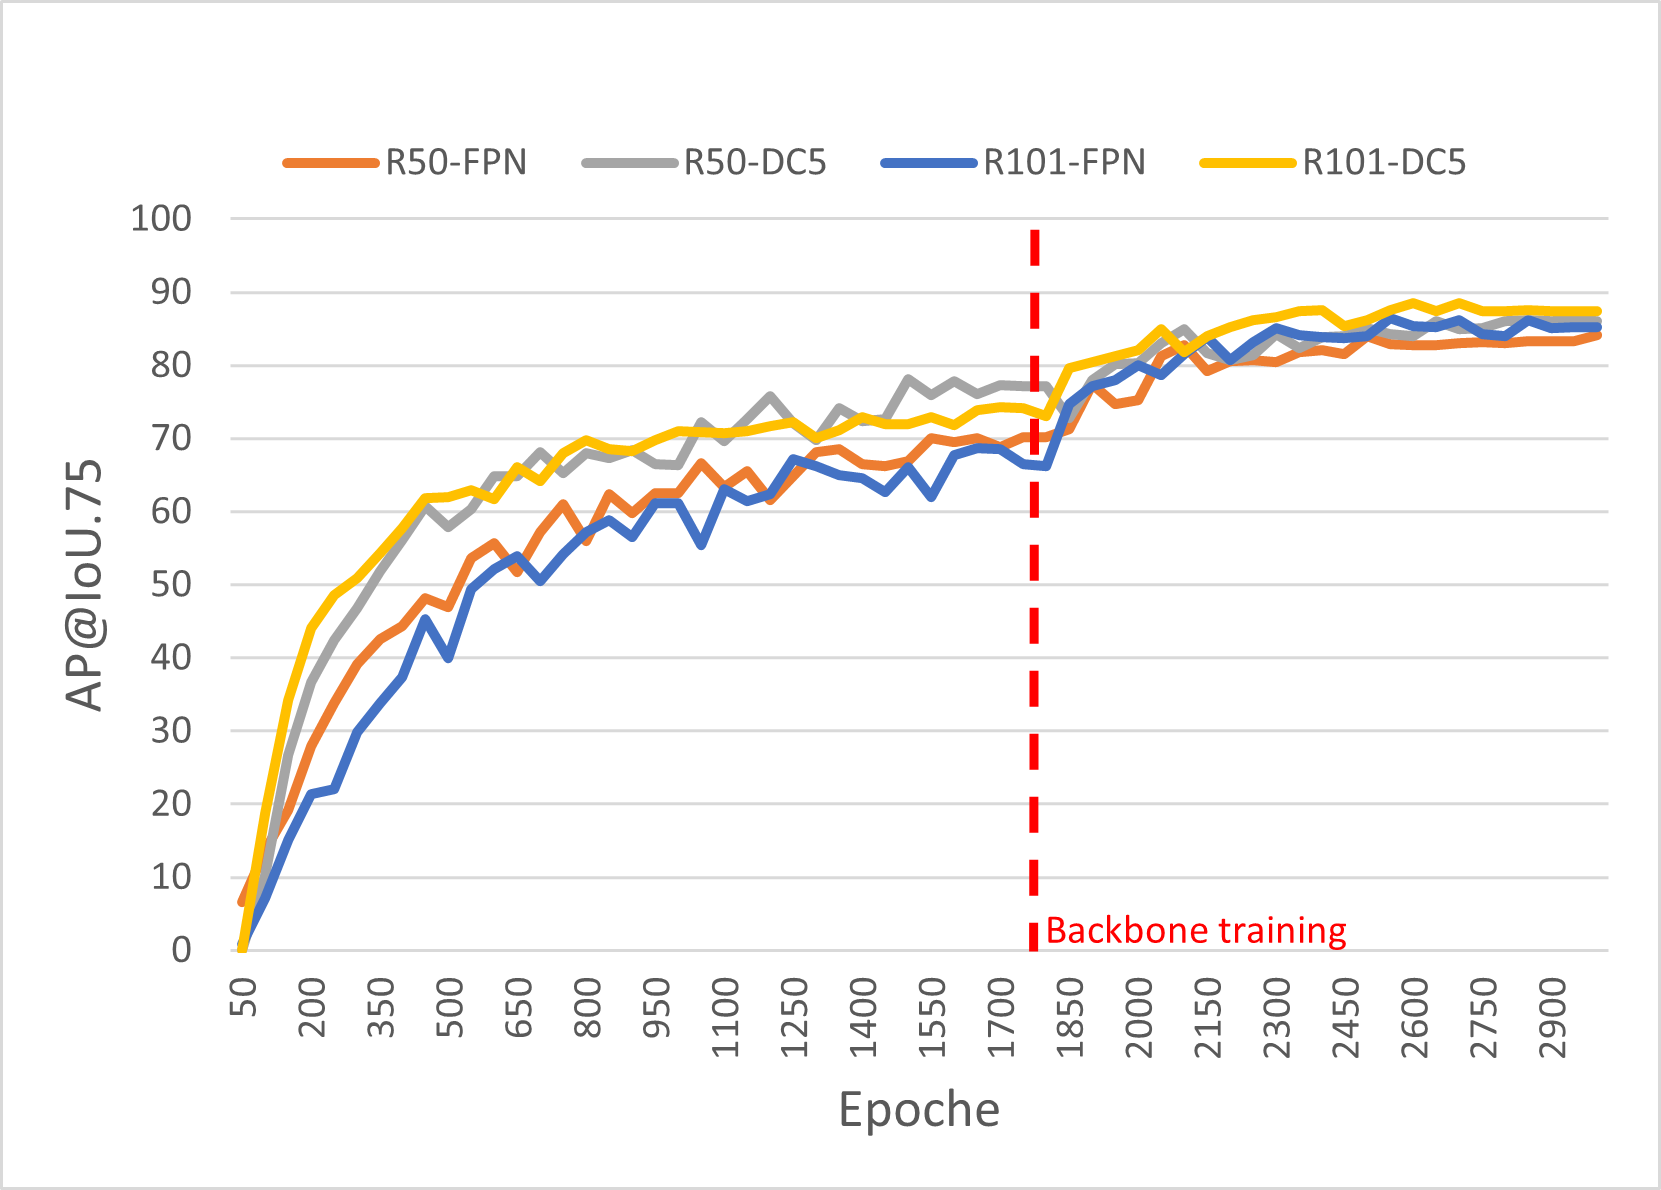
\includegraphics{img/eval/bboxap75.png}
%     \caption{AP der Bounding Box Vorhersage bei einem IoU-Wert von 0,75 für die verschiedenen Backbones während der Trainingsepisoden. Es ist zu erkennen, dass die AP nach ca. 1800 Epochen konvergiert, aber eine weitere Steigerung erfährt, sobald das Backbone-Training aktiviert wird. Diese Grafik zeigt die Entwicklung der Modellleistung während des Trainingsprozesses.}
%     \label{tab:bboxap75}
% \end{figure}

% \begin{table}[htbp]
% \centering
% \begin{tabular}{lrrr}
% \toprule
% Backbone & $\text{AP}$ & $\text{AP}^{IoU=.5}$ & $\text{AP}^{IoU=.75}$\\
% \midrule
% ResNet-50-FPN & 71.84 & 89.79 & 83.48 \\
% ResNet-50-C5-dilated & \textbf{77.21} & \textbf{93.65} & \textbf{86.11}\\
% ResNet-101-FPN & 75.13 & 92.71 & 85.39\\
% ResNet-101-DC5 & 77.85 & 94.44 & 87.47\\
% \bottomrule
% \end{tabular}
% \caption{AP Werte der Bounding-Box-Vorhersage, bei unterschiedlichen IoU Werten für die verschiedenen Modellvarianten. Mittelwert der letzten 200 Epochen.}
% \label{tab:bboxap}
% \end{table}
\section{Auswertung auf dem Validierungsdatensatz}
\begin{figure}[h]
    \centering
    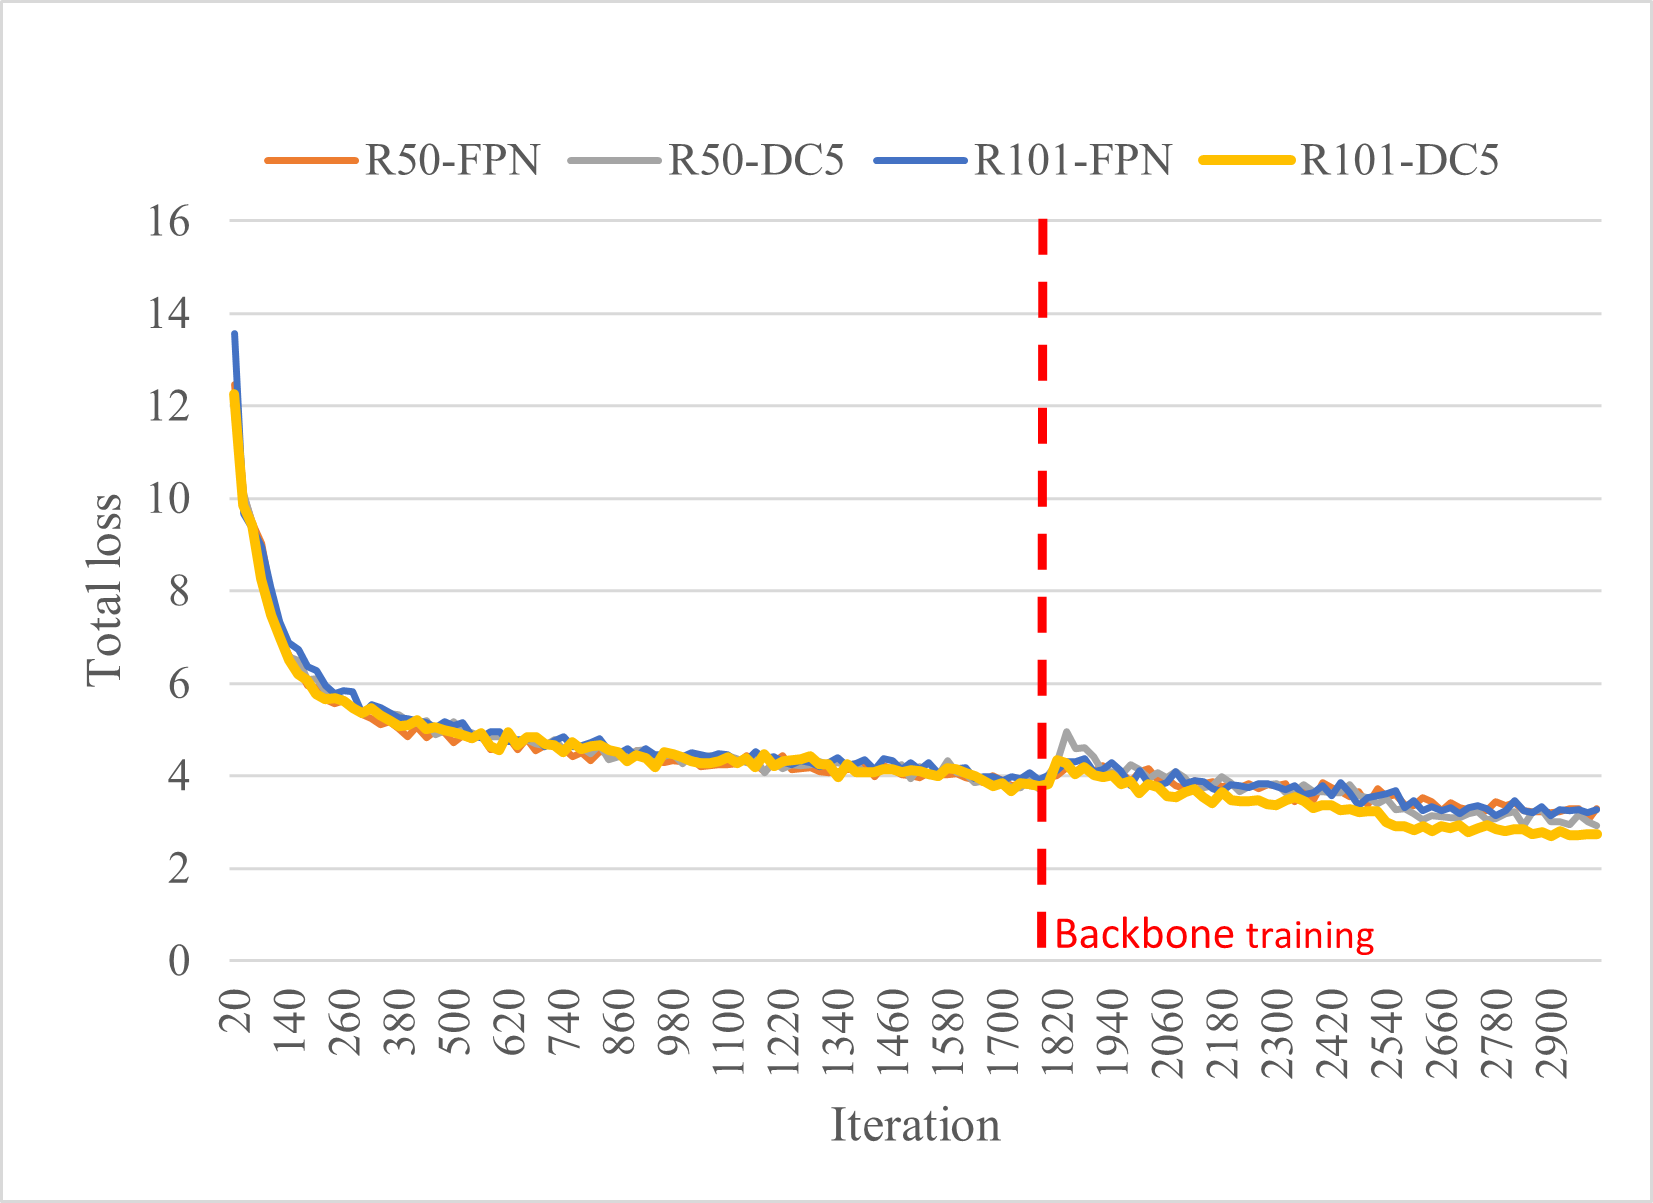
\includegraphics[]{img/eval/total_loss.png}
    \caption{Gesamter Fehler der Modelle über die Trainingsepochen. Bei Iteration 1800 beginnt das training des Backbones.}
    \label{fig:loss}
\end{figure}
Die Abbildung \ref{fig:loss} zeigt den Gesamtfehler der trainierten Netze über die Epochen. Sie zeigt eine stabile Konvergenz aller Modelle ohne signifikante Sprünge, mit Ausnahme eines vorübergehenden Fehleranstiegs nach Iteration 1800, als das Training des Backbones zur Verfeinerung der Merkmalsextraktion beginnt. Die Kurven der verschiedenen Modelle überlagern sich, was auf ein ähnliches Lernverhalten hindeutet.
\clearpage
\subsection{Ergebnisse der Segmentierung}
\begin{table}[htbp]
\centering
\begin{tabular}{lrrr}
\toprule
Backbone & $\text{AP}$ & $\text{AP}^{IoU=.5}$ & $\text{AP}^{IoU=.75}$\\
\midrule
ResNet-50-FPN & 47.80 & 84.68 & 46.08 \\
ResNet-50-DC5 & 53.92 & \textbf{89.22} & \textbf{60.23}\\
ResNet-101-FPN & 50.39 & 88.62 & 51.01\\
ResNet-101-DC5 & \textbf{54.33} & 89.05 & 59.24\\
\bottomrule
\end{tabular}
\caption{Mittelwert der letzten 200 Epochen von $\text{AP}$, $\text{AP}^{IoU=.5}$, $\text{AP}^{IoU=.75}$ der Segmentierung für die verschiedenen Modelle.}
\label{tab:segap75}
\end{table}
\begin{figure}[h]
    \centering
    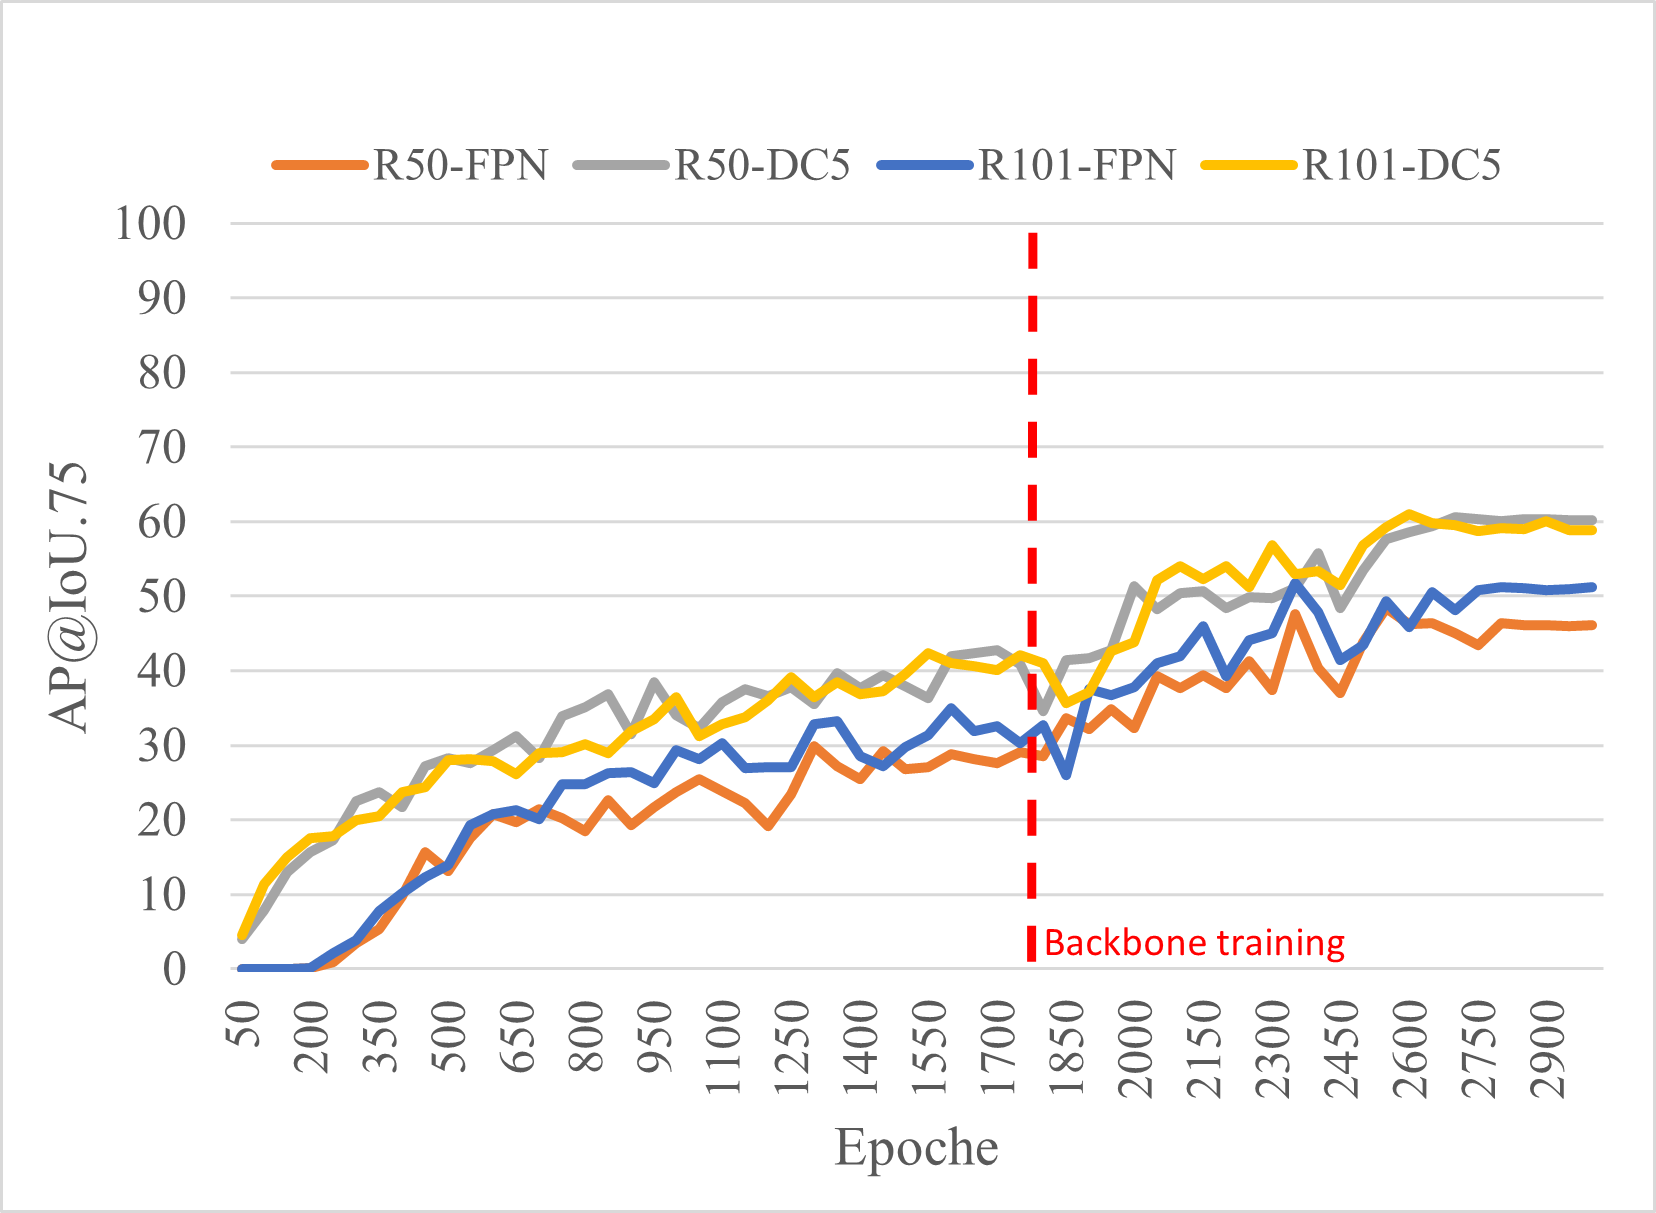
\includegraphics[trim={.3cm .25cm .2cm 1cm}, clip]{img/eval/segap75.png}
    \caption{Entwicklung der $\text{AP}^{IoU=.75}$ für die verschiedenen Backbones während der Trainingsepisoden.}
    \label{fig:segap75}
\end{figure}
Die AP-Werte der Segmentierung für verschiedene IoU-Werte, aufgeschlüsselt nach verschiedenen Backbone-Varianten sind in Tabelle \ref{tab:segap75} dargestellt. Bei den ResNet-50-Backbones ist ein Anstieg der AP um ca. fünf Prozent beim Wechsel von FPN zu DC5 zu beobachten. Dieser Trend ist bei allen AP-Varianten zu beobachten. Ähnliche Verbesserungen zeigen sich auch beim Wechsel von FPN zu DC5 in den ResNet-101-Backbones, insbesondere bei der strengen Metrik $\text{AP}^{IoU=.75}$, wo ein Anstieg von über acht Prozent gemessen wird. Auffällig ist, dass die Genauigkeit der Segmentierung zwischen den Netzwerken ResNet-50-DC5 und ResNet-101-DC5 nur einen Unterschied von weniger als einem Punkt aufweist.

Aus Abbildung \ref{fig:segap75} wird deutlich, dass die DC5-Varianten der Netze bereits nach 50 Epochen einen Trainingseffekt aufweisen. Im Gegensatz zur FPN-Variante, die erst nach 200 Epochen Vorhersagen liefert.  Über den gesamten Trainingszeitraum erreichen die DC5-Varianten eine höhere $\text{AP}^{IoU=.75}$ als die FPN-Varianten. Eine erkennbare Konvergenz aller Netze tritt nach 1800 Epochen auf. Die Aktivierung des Backbone-Trainings führt jedoch zu einem weiteren Anstieg der AP-Werte.


\subsection{Ergebnisse der Keypoint-Vorhersage}
\begin{table}[h]
\centering
\begin{tabular}{lrrr}
\toprule
Backbone & $\text{AP}$ & $\text{AP}^{OKS=.5}$ & $\text{AP}^{OKS=.75}$\\
\midrule
ResNet-50-FPN & 90.74 & 91.94 & 90.79 \\
ResNet-50-DC5 & 94.88 & 95.08 & 95.08\\
ResNet-101-FPN & 93.40 & 93.78 & 93.67\\
ResNet-101-DC5 & \textbf{95.24} & \textbf{95.34} & \textbf{95.34}\\
\bottomrule
\end{tabular}
\caption{$\text{AP}$, $\text{AP}^{OKS=.5}$, $\text{AP}^{OKS=.75}$ Werte der Keypoint-Vorhersage für die verschiedenen Modelle.}
\label{tab:keyap75}
\end{table}

\begin{figure}[h]
    \centering
    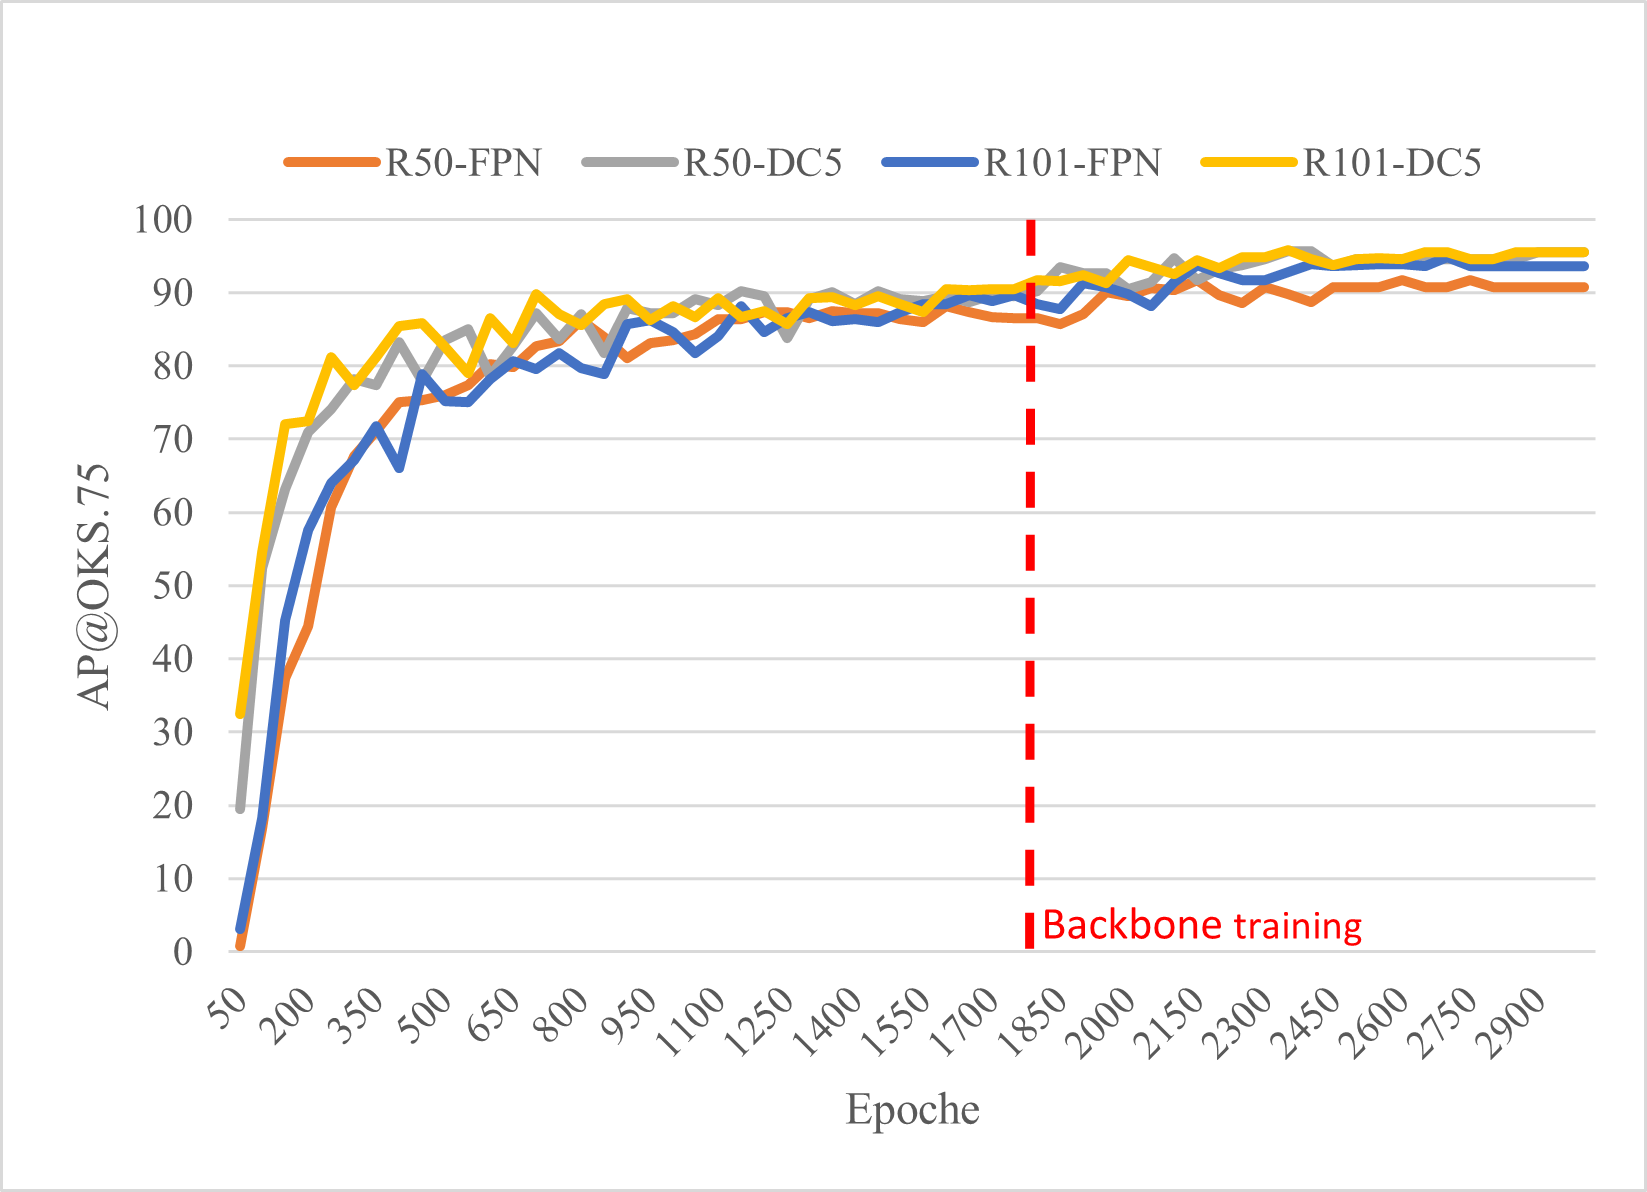
\includegraphics[trim={.3cm .25cm .2cm 1cm}, clip]{img/eval/keyap75.png}
    \caption{Darstellung der $\text{AP}^{OKS=.75}$ der Keypoint-Vorhersage für die verschiedenen Backbones über die Trainingsepisoden.}
    \label{fig:keyap75}
\end{figure}
Die in Tabelle \ref{tab:keyap75} und Abbildung \ref{fig:keyap75} dargestellten AP-Werte bei unterschiedlichen OKS-Werten, geben einen wertvollen Einblick in die Leistungsfähigkeit verschiedener Backbone-Modelle im Kontext der Key-Point-Vorhersage. Der steile Anstieg der $\text{AP}^{OKS=.75}$ in den ersten 300 Epochen deutet darauf hin, dass alle Netze bereits nach wenigen Trainingsepochen die ungefähre Position des Apex der Spitze lernen. Ein stetiger Anstieg der Genauigkeit ist in den folgenden Epochen zu beobachten, bis die Netze um Epoche 1500 konvergieren. Ein weiterer kleiner, aber signifikanter Lerneffekt tritt mit dem Backbone-Training nach Epoche 1800 auf.

Die endgültigen AP-Werte, die in Tabelle \ref{tab:keyap75} dargestellt sind, unterscheiden sich bei der Keypoint-Erkennung zwischen den Netzen nur um wenige Prozent, aber jede Verbesserung ist hier entscheidend. Insbesondere die Verwendung von DC5 anstelle von FPN führt zu einer deutlichen Verbesserung, wobei ResNet-101-DC5 in allen AP-Varianten die höchste Genauigkeit erreicht. Dies deutet auf eine überlegene Genauigkeit dieses Modells bei der Vorhersage von Schlüsselpunkten hin.
Auch die Modelle ResNet-50-FPN und ResNet-101-FPN erreichen mit über 90 Prozent ebenfalls respektable Werte, insbesondere das Modell ResNet-50-DC5, dessen Leistung bis auf weniger als einen Punkt an die von ResNet-101-DC5 heranreicht. Dies legt nahe, dass diese Modelle trotz ihrer Unterlegenheit als robuste Optionen für Aufgaben mit geringeren Genauigkeitsanforderungen in Betracht gezogen werden könnten.

\section{Fehlerhafte Vorhersagen}
\begin{table}[h]
\centering
\begin{tabular}{lcc}
\toprule
Backbone & $FN$ & $FP$ \\
\midrule
ResNet-50-FPN & 0.0937 & 0.0597 \\
ResNet-50-DC5 & 0.0819 & 0.0429 \\
ResNet-101-FPN & 0.0941 & 0.0536 \\
ResNet-101-DC5 & \textbf{0.0780} & \textbf{0.0390} \\
\bottomrule
\end{tabular}
\caption{Falsch-negativ und falsch-positiv Raten von Mask R-CNN mit verschiedenen Backbones.}
\label{tab:fnfp}
\end{table}
\begin{figure}[h]
    \centering
    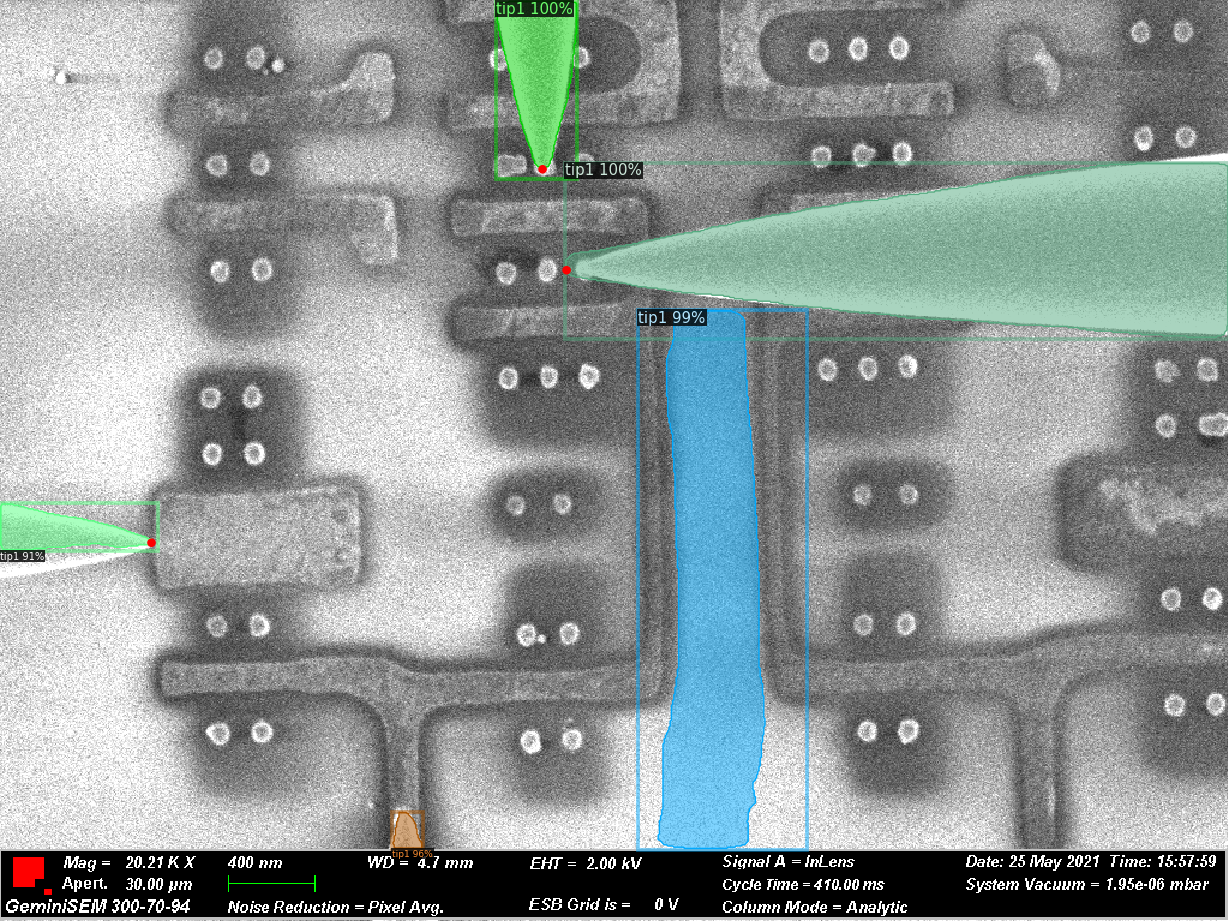
\includegraphics[width=0.5\linewidth]{img/eval/images/r50-fpn-false.png}
    \caption{Visualisierung der Detektionen des ResNet-50-FPN-Netzes mit einem Konfidenzschwellenwert von 90\%.}
    \label{fig:falsepos}
\end{figure}
Tabelle \ref{tab:fnfp} zeigt die FN- und FP-Raten der verschiedenen Netze. Wie eingangs erwähnt, spielen neben der Genauigkeit der Keypoint-Erkennung auch die FN- und FP-Raten eine entscheidende Rolle, da falsche Detektionen zu erheblichen Schäden führen können.

Alle Netze erreichen eine FN-Rate von unter zehn Prozent, das heißt von 100 Spitzen werden weniger als 10 Nadeln nicht erkannt. Die FP-Rate, ein Indikator dafür, wie viele spitzen ähnliche Strukturen das Netz als Spitze identifiziert, obwohl keine vorhanden ist, liegt bei allen Netzen unter 6 Prozent.
Die DC5-Varianten der Backbones zeigen erneut ihre Überlegenheit, da sie in allen Fällen um etwa eineinhalb Prozent niedrigere Werte erreichen. Das ResNet-101-DC5-Backbone schneidet von allen Kombinationen am besten ab, wenn auch nur mit geringem Abstand.

Es ist zu beachten, dass eine Verringerung der FN-Rate durch Herabsetzung des Konfidenzschwellenwertes zwangsläufig zu einer Erhöhung der FP-Rate führt und umgekehrt. Daher muss ein angemessenes Gleichgewicht zwischen diesen beiden Raten gefunden werden, das den spezifischen Anforderungen der jeweiligen Aufgabe entspricht.
Die Abbildung \ref{fig:falsepos} veranschaulicht diese Abwägung anhand eines Beispiels. Die falsch-positive Detektion, hier in hellblau dargestellt, hat eine Konfidenz von 99\%. Die Detektionen von Spitze 7 (West) und 5 (Süd) haben eine Konfidenz von 91\% beziehungsweise 96\%. Beachtlich ist die Detektion
der Spitze 5. Wenn der Schwellenwert auf 99\% erhöht wird, sinkt die FP-Rate, aber die FN-Rate steigt. Diese Darstellung verdeutlicht die notwendige Abwägung zwischen der Minimierung von falsch-positiven und falsch-negativen Detektionen.
\section{Vorhersage mit Spitzenrichtung}
In diesem Abschnitt wird die Leistung der Modelle ResNet-50-DC5 und ResNet-101-DC5 untersucht, die so trainiert wurden, dass sie die Spitzen je nach ihrer Richtung als acht verschiedene Klassen behandeln. Ziel dieser Modifikation ist es, nicht nur das Vorhandensein von Spitzen, sondern sie auch anhand ihrer Richtung zu klassifizieren.

\begin{figure}[h]
    \centering
    \subfigure[ResNet-50-DC5]{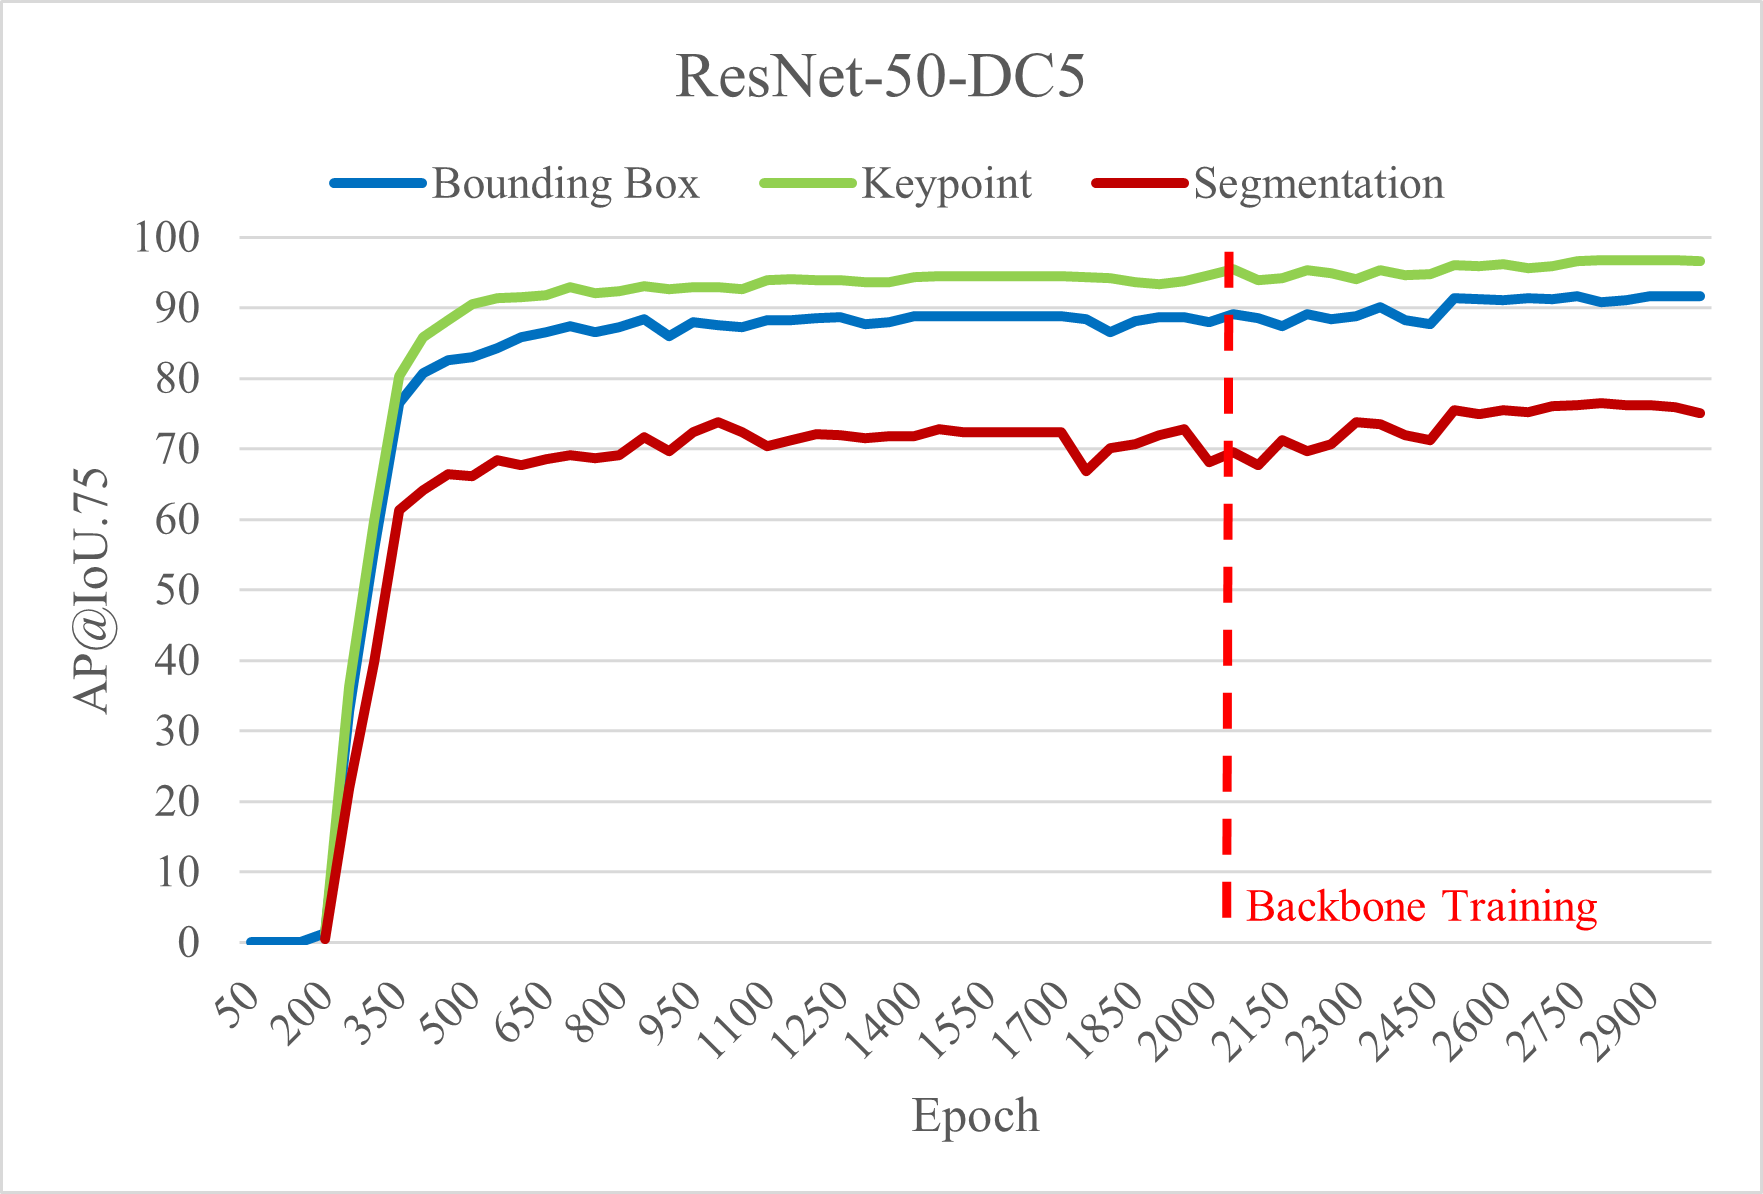
\includegraphics[width=0.49\textwidth, trim=.5cm .4cm .6cm 1cm, clip]{img/eval/r50-dc5-ap75_multiclass.png}}
    \subfigure[ResNet-101-DC5]{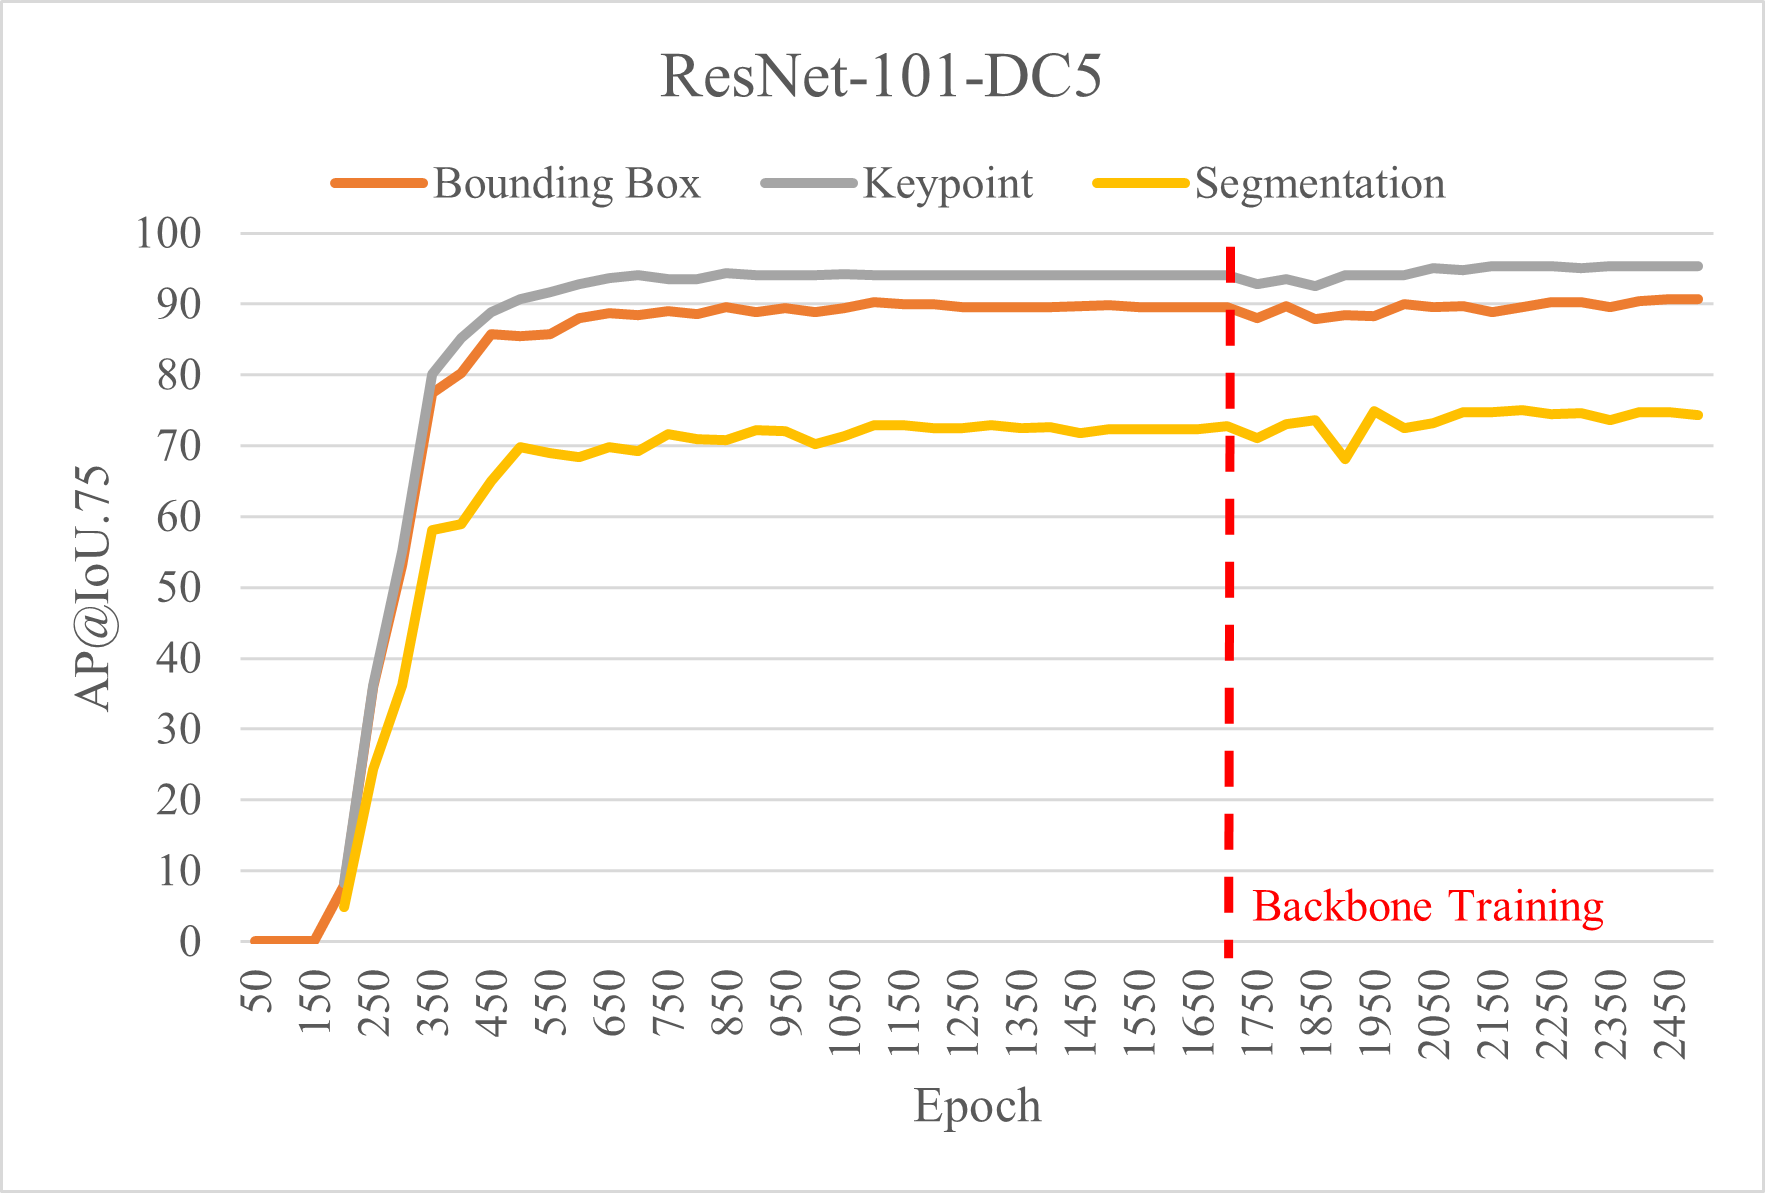
\includegraphics[width=0.49\textwidth, trim=.5cm .4cm .6cm 1cm, clip]{img/eval/r101-dc5-ap75_multiclass.png}}
    \caption{$\text{AP}^{.75}$-Werte für die Bounding-Box-Vorhersage, die Segmentierung und die Keypoint-Erkennung. Für die Modelle, welche die Spitzen anhand ihrer Richtung unterscheiden.}
    \label{fig:ap75-mc}
\end{figure}

\begin{table}[h]
\centering
\begin{tabular}{lrrrrr}
\toprule
Backbone & $\text{AP}^{IoU=.75}_{BB}$ & $\text{AP}^{IoU=.75}_{S}$ & $\text{AP}^{OKS=.75}_{K}$ & $FN$ & $FP$\\
\midrule
ResNet-50-DC5 & 86.11 & 60.23 & 95.08 & 0.0819 & 0.0429 \\
ResNet-50-DC5-Multiclass & 89.52 & \textbf{75.53} & 95.18 & 0.0617 & 0.0301 \\
\hline
ResNet-101-DC5 & 87.45 & 59.24 & 95.34 & 0.0780 & 0.0390 \\
ResNet-101-DC5-Multiclass & \textbf{90.33} & 74.34 & \textbf{95.34} & \textbf{0.055} & \textbf{0.023} \\
\bottomrule
\end{tabular}
\caption{Vergleich der Werte $\text{AP}^{IoU=.75}_{BB}$, $\text{AP}^{IoU=.75}_{S}$, $\text{AP}^{OKS=.75}_{K}$ des auf ein oder acht Klassen trainierten Modells. Aufgeteilt nach Backbone-Architektur.}
\label{tab:multiclass}
\end{table}
\begin{figure}[h]
    \centering
    \subfigure[ResNet-50-DC5]{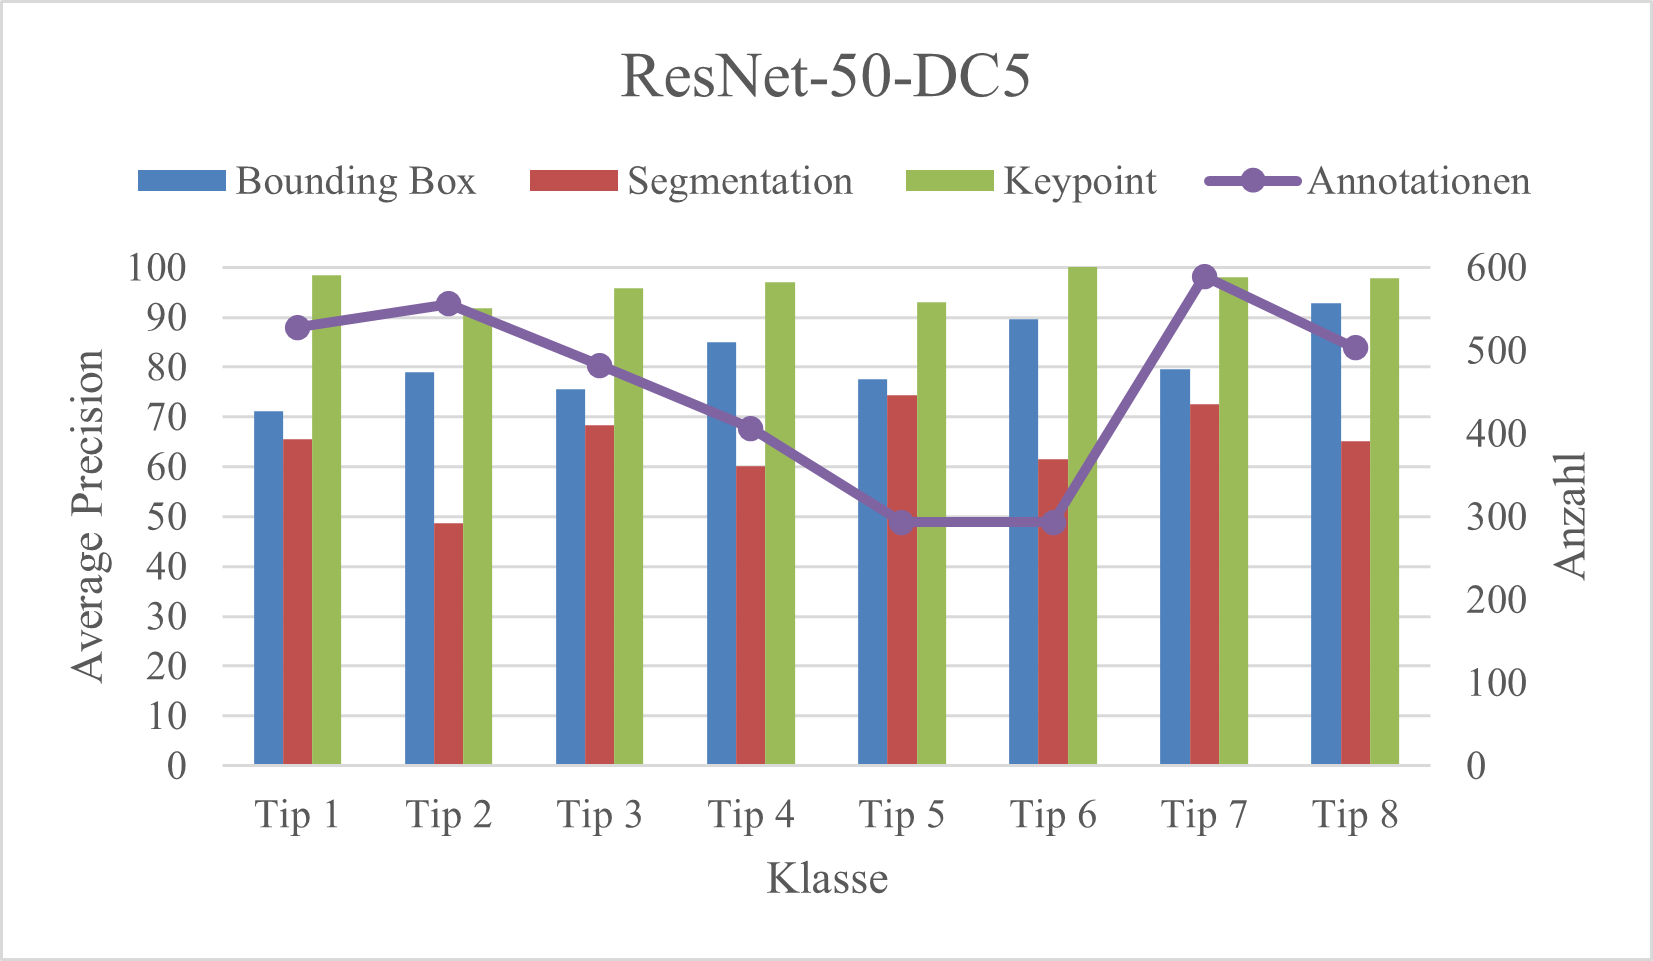
\includegraphics[width=0.49\textwidth, trim=.5cm .4cm .45cm 1cm, clip]{img/eval/r50-dc5_correlation.png}}
    \subfigure[ResNet-101-DC5]{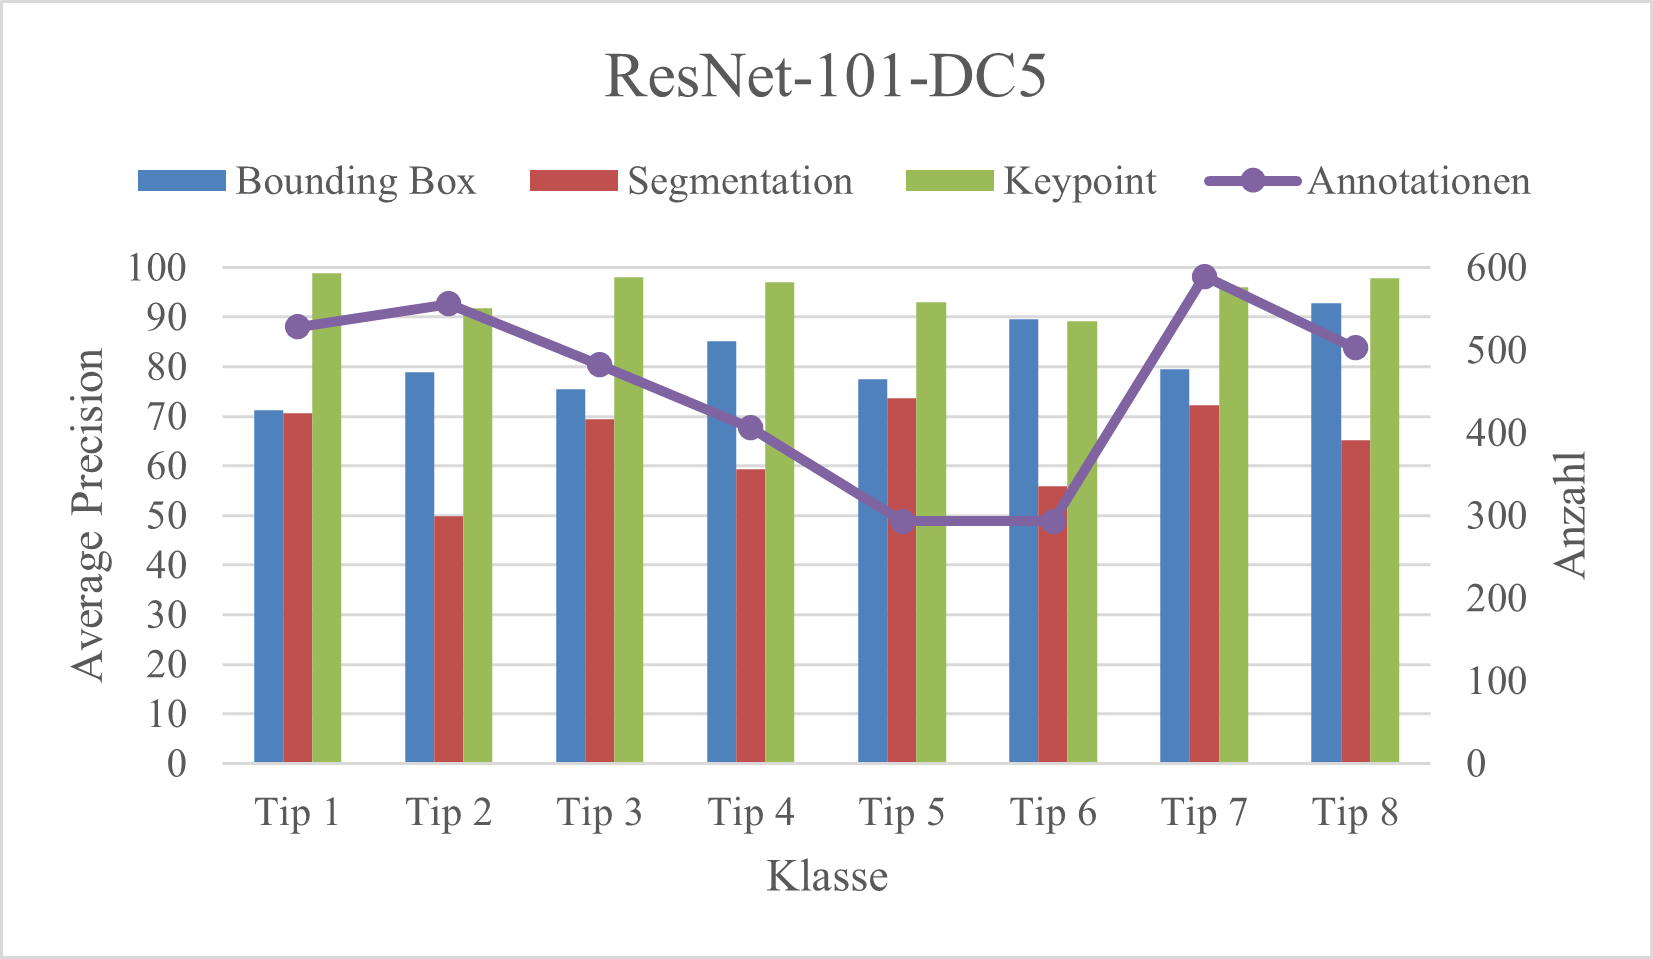
\includegraphics[width=0.49\textwidth, trim=.5cm .4cm .45cm 1cm, clip]{img/eval/r101-dc5_correlation.png}}
    \caption{$\text{AP}^{.75}$-Werte der Vorhersagen, getrennt nach den acht Klassen und die Anzahl der Instanzen pro Klasse im Trainingsdatensatz. Es wird eine mögliche Korrelation zwischen der Menge der Trainingsdaten und der Vorhersagegenauigkeit untersucht.}
    \label{fig:correl}
\end{figure}
In Abbildung \ref{fig:ap75-mc} ist der Fortschritt der Modelle während des Trainingsprozesses dargestellt. Beide Modelle zeigten einen steilen Anstieg der Vorhersagegenauigkeit um die 300. Epoche und beginnen bereits nach circa 400 Epochen zu konvergieren. Das weitere Training der Backbones ab Epoche 1700 führt zunächst zu einer Instabilität der Modelle, die sich jedoch wieder ausgleicht und die Gesamtleistung nur marginal verbesserte. Dies bestätigt die Annahme, dass das auf einer Klasse vortrainierte Backbone die Eigenschaften der Spitzen bereits optimal extrahiert.

Eine deutliche Steigerung zeigt sich bei der Genauigkeit der Segmentierung beider Modelle. Tabelle \ref{tab:multiclass} zeigt, dass die Modelle im Vergleich zu den zuvor trainierten Varianten einen Zuwachs von etwa 15 Prozent verzeichnen. Dies deutet auf eine verbesserte Fähigkeit der Modelle hin, die Struktur und Position der Nadelspitzen genauer zu erkennen.
Bemerkenswert ist die drastische Reduzierung der FN- und FP-Raten um 40 Prozent. Dies zeigt, dass die Modelle nicht nur besser in der Lage sind, echte Nadelspitzen korrekt zu identifizieren, sondern auch weniger dazu neigen, andere Strukturen fälschlicherweise als solche zu interpretieren. Das Modell macht also weniger Fehler, sowohl bei übersehenen als auch bei fälschlich identifizierten Spitzen.
Die Genauigkeit der Schlüsselpunkt-Vorhersage bleibt unverändert.

\begin{table}[h]
    \centering
    \begin{tabular}{lrrr|rrr}
        \toprule
         & \multicolumn{3}{c}{ResNet-50-DC5} & \multicolumn{3}{c}{ResNet-101-DC5} \\
        Korrelation & $\text{AP}^{IoU=.75}_{BB}$ & $\text{AP}^{IoU=.75}_{S}$ & $\text{AP}^{OKS=.75}_{K}$ & $\text{AP}^{IoU=.75}_{BB}$ & $\text{AP}^{IoU=.75}_{S}$ & $\text{AP}^{OKS=.75}_{K}$ \\
        \midrule
        Trainingsbilder & 0,159 & 0,169 & 0,741 & -0,089 & 0,047 & 0,526\\
        Eckposition & -0,776 & 0,681 & -0,220 & -0,727 & 0,864 & 0,384\\ 
        \bottomrule
    \end{tabular}
    \caption{Berechnete Korrelationskoeffizienten zwischen der Anzahl der Trainingsbilder pro Spitze und der Genauigkeit des Modells sowie zwischen der Eckposition der Spitzen und der Genauigkeit.}
    \label{tab:correl}
\end{table}
Die Unterteilung der Spitzen in acht Klassen ermöglicht es, den Zusammenhang zwischen der Anzahl der Instanzen der Spitzen in den Trainingsbildern und der Leistungsfähigkeit der Modelle zu analysieren. Wie bereits in Abbildung \ref{fig:instpclass} dargestellt, sind insbesondere die Spitzen 5 (Süd) und 6 (Süd-West) unterrepräsentiert.

Abbildung \ref{fig:correl} veranschaulicht die Leistung der Modelle auf den verschiedenen Klassen und die Klassenverteilung des Trainingsdatensatzes. Für eine quantitative Analyse wird die Korrelation zwischen der Modellleistung und der Anzahl der Instanzen der jeweiligen Klassen berechnet.
Auffällig ist dabei, dass $\text{AP}^{OKS=.75}_{K}$ eine hohe positive Korrelation aufweist. Das kann bedeuten, dass je mehr Bilder von einer Spitze für das Training zur Verfügung stehen, desto genauer ist die Keypoint-Vorhersage. Die erzeugten Segmentierungen und Bounding Boxen zeigen jedoch nur für ResNet-50-DC5 eine schwache Korrelation.

Besonders interessant ist die starke Korrelation zwischen der Position einer Spitze (ob sie aus einer Ecke in das Bild hineinragt) und der Genauigkeit der Bounding Box und der Segmentierung. Die Genauigkeit der Bounding Box $\text{AP}^{IoU=.75}_{BB}$ korreliert positiv mit der Eckposition. Dies ist darauf zurückzuführen, dass die Bounding Box bei schrägen Objekten per Definition größer ist, da sich nicht eng anliegt. Dies hat zur Folge, dass bei einer festen IoU eine größere Abweichung toleriert wird, was die berechnete Genauigkeit erhöht.
Andererseits korreliert die Genauigkeit der Segmentierung negativ mit der Eckposition. Dies deutet darauf hin, dass die Netze Schwierigkeiten bei der Segmentierung von schrägen Nadeln haben, dies wird im folgenden Kapitel \ref{sec:optkon} durch die optische Überprüfung bestätigt.

\clearpage
\section{Optische Überprüfung}
\label{sec:optkon}
Trotz der Bedeutung der quantitativen Metriken ist die qualitative Bewertung der Modellvorhersagen ebenso wichtig, um eine Gesamtbeurteilung der Modellleistung zu erhalten. Zu diesem Zweck werden dem Modell 100 nicht annotierte Bilder vorgelegt und die Ergebnisse manuell überprüft.
Diese Methode ermöglicht eine intuitive und praktische Bewertung der Modellgenauigkeit. Beispielsweise können Muster von Fehlern oder Ungenauigkeiten identifiziert werden, die durch quantitative Metriken möglicherweise übersehen werden. Darüber hinaus bietet die visuelle Verifikation die Möglichkeit, die Qualität der Modellvorhersagen im Kontext realer Anwendungen zu beurteilen, was letztlich ein entscheidendes Kriterium für die Nützlichkeit des Modells ist.

Die Ergebnisse dieser Überprüfung und ihre Bedeutung für die Modellleistung und -auswahl werden in den folgenden Abschnitten ausführlich dargestellt und diskutiert.
Alle Bilder werden von den Modellen bei einem Konfidenzschwellwert von 99\% analysiert, was eine hohe Sicherheit der Modellvorhersagen erfordert.

\newpage

\begin{figure}[h!]
    \centering
    \subfigure[ResNet-50-FPN]{\label{subfig:r50-fpn-img1}
    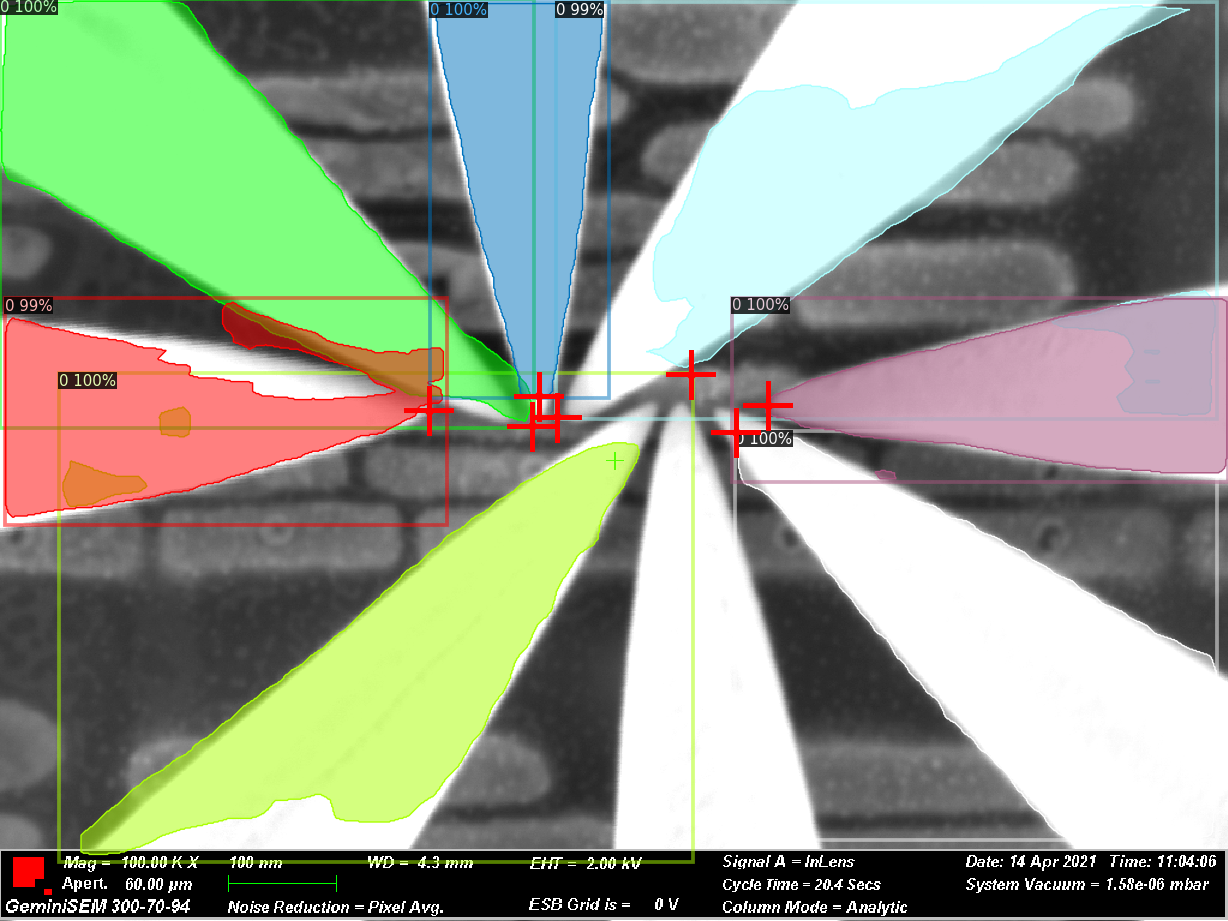
\includegraphics[width=0.485\textwidth]{img/eval/images/r50-fpn-image_003.png}}
    \subfigure[ResNet-50-DC5]{\label{subfig:r50-dc5-img1}
    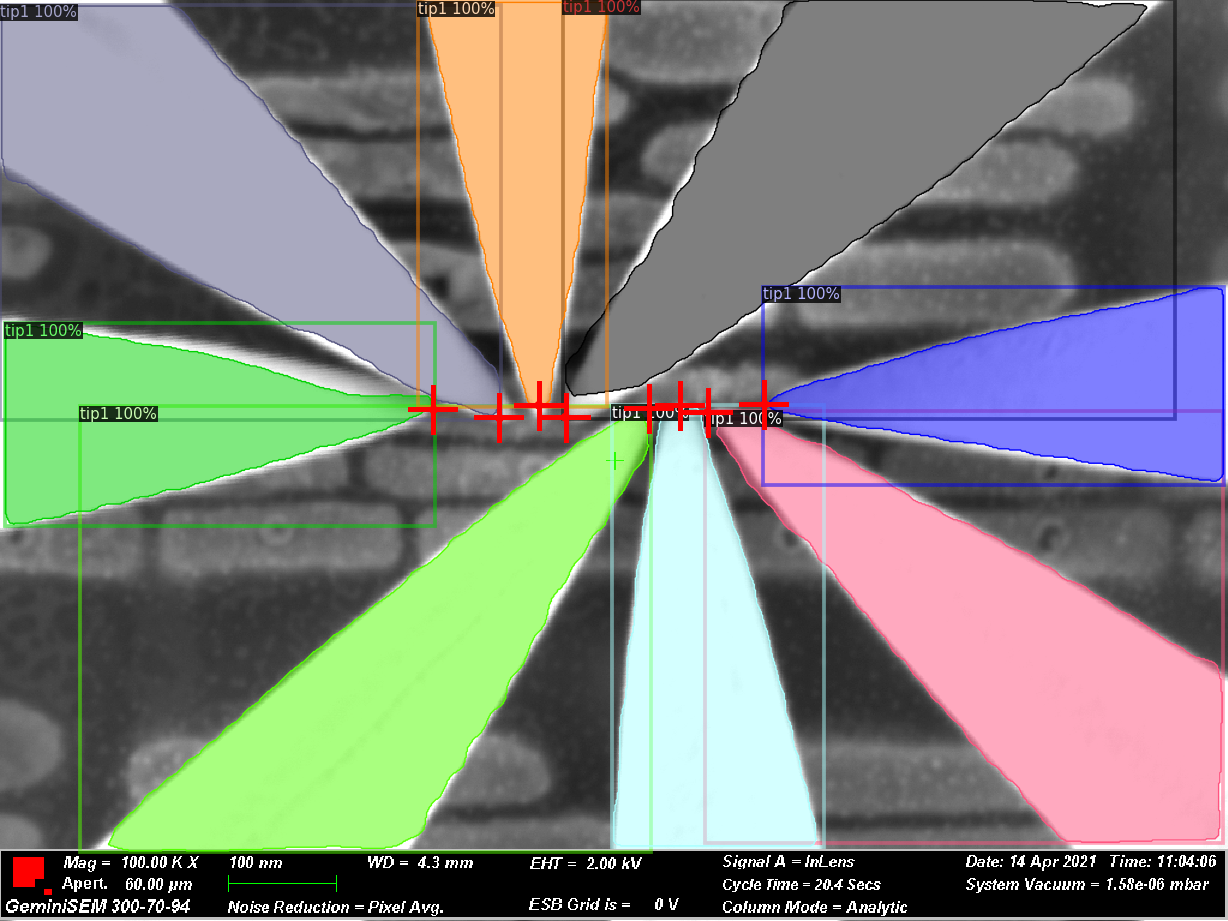
\includegraphics[width=0.485\textwidth]{img/eval/images/r50-dc5-image_003.png}}
    \subfigure[ResNet-101-FPN]{\label{subfig:r101-fpn-img1}
    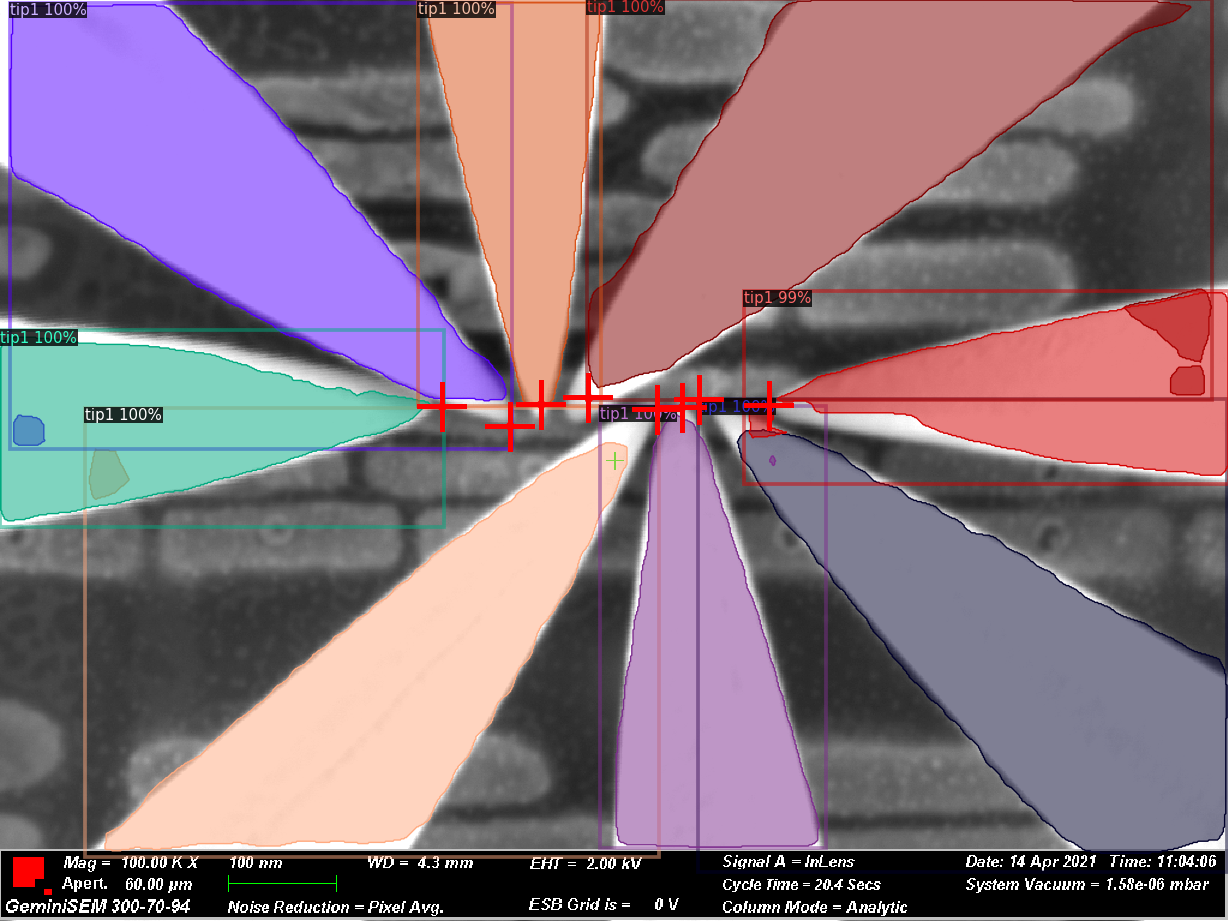
\includegraphics[width=0.485\textwidth]{img/eval/images/r101-fpn-image_003.png}}
    \subfigure[ResNet-101-DC5]{\label{subfig:r101-dc5-img1}
    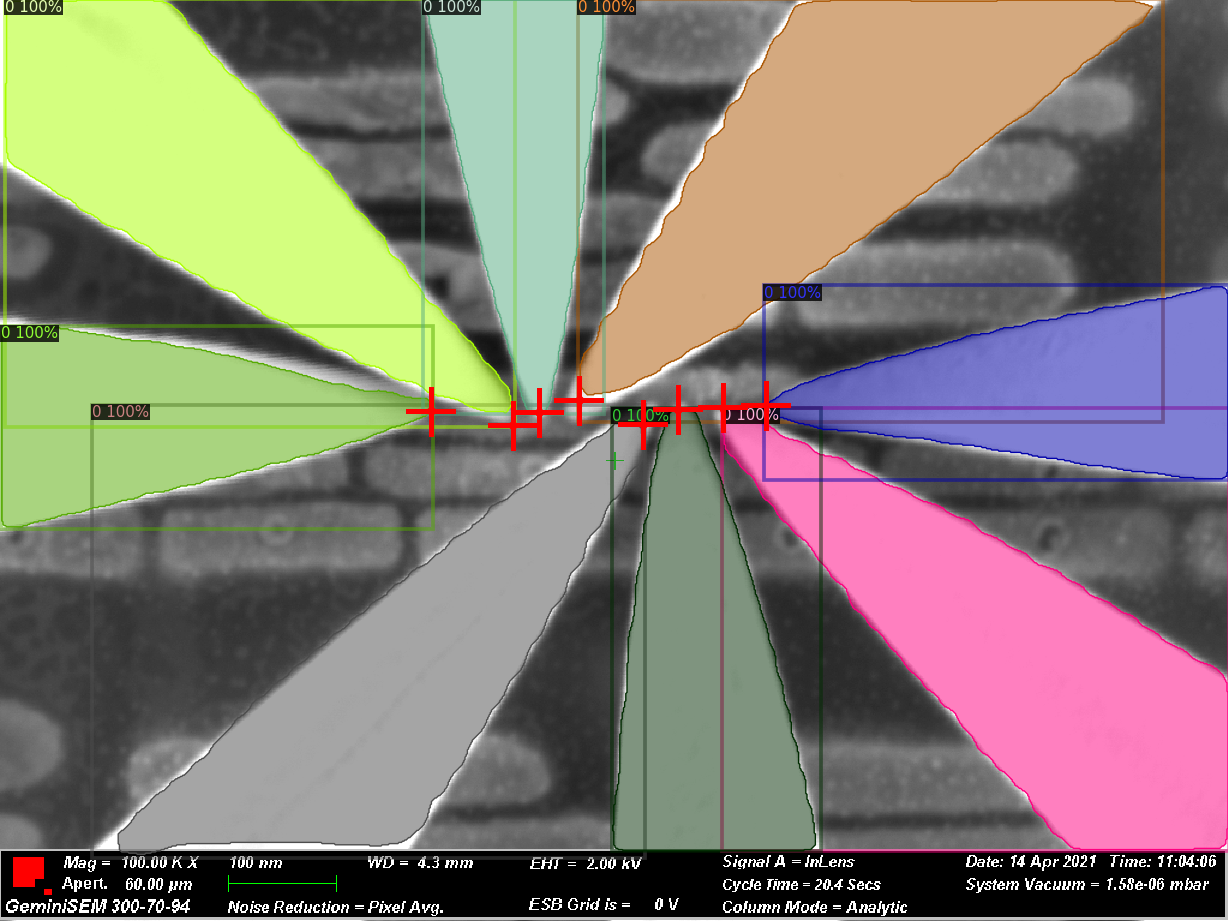
\includegraphics[width=0.485\textwidth]{img/eval/images/r101-dc5-image_003.png}}
    \caption{Acht Spitzen beim Kontaktieren einer Probe. Aufgenommen bei 100.000-facher Vergrößerung. Die Segmentierung der jeweiligen Netze ist über das Bild gelegt.}
    \label{fig:comp_img1}
\end{figure}
Bei der Untersuchung von Segmentierungsmasken und Keypoint-Vorhersagen für Bilder mit einer Vergrößerung von mehr als 30.000x – Bedingungen, die typischerweise während des Probings auftreten – zeigt sich, dass nur die FPN-Varianten falsch-positive Detektionen liefern, während die DC5-Varianten durchweg korrekte Detektionen enthält.
Auffällig ist auch, dass die auf dem FPN-Backbone basierenden Modelle eine unsaubere Segmentierung erzeugen, die durch die Bildung von Artefakten gekennzeichnet ist. Diese Artefakte treten in der Form auf, dass Teile anderer Spitzen oder des Hintergrundes fälschlicherweise der Spitze zugeordnet werden oder ein Teil der Spitze überhaupt nicht erkannt wird. Zudem sind die Keypoints des ResNet-50-FPN oft nicht exakt gesetzt. Teilweise liegen sie neben der Spitze oder sind zu weit nach hinten versetzt. Im Gegensatz dazu zeigen die DC5-Varianten der Modelle keine Artefakte. Sie segmentierten die Spitzen mit hoher Genauigkeit und auch die Keypoints scheinen zuverlässig erkannt zu werden.

In Abbildung \ref{fig:comp_img1} ist ein Szenario zu sehen, in dem die Beobachtungen zum Teil ebenfalls auftreten.
Es wird auch beobachtet, dass alle Modelle Schwierigkeiten haben, wenn nur ein kleiner Teil der Spitze sichtbar ist. Eine weitere interessante Beobachtung betrifft allerdings alle Modelle gleichermaßen: Die Konturen der Segmentierungen der in den Ecken liegenden Spitzen (Spitze 2, 4, 6, 8) erscheint wellig.

\begin{figure}[h!]
    \centering
    \subfigure[ResNet-50-FPN]{\label{subfig:r50-fpn-img2}
    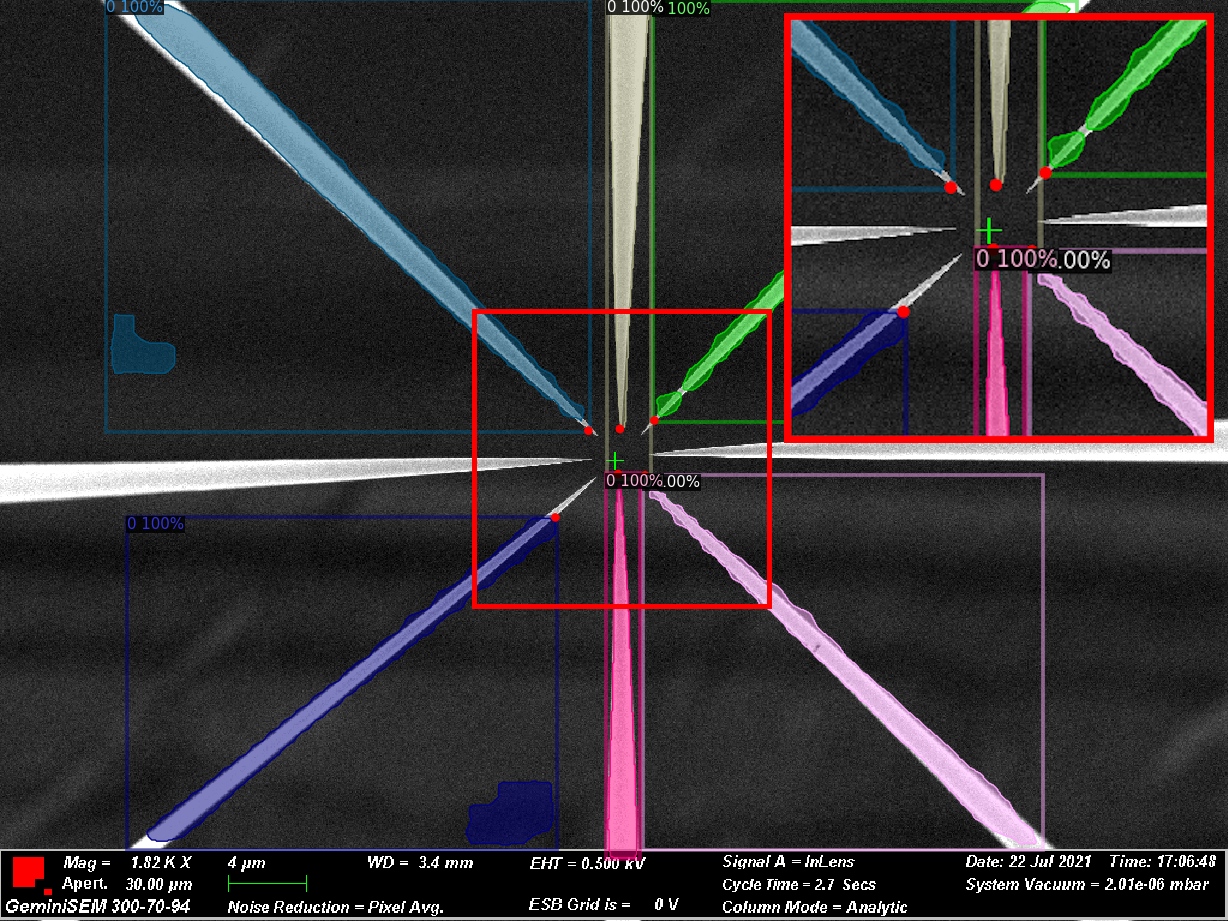
\includegraphics[width=0.485\textwidth]{img/eval/images/r50-fpn-image__004.png}}
    \subfigure[ResNet-50-DC5]{\label{subfig:r50-dc5-img2}
    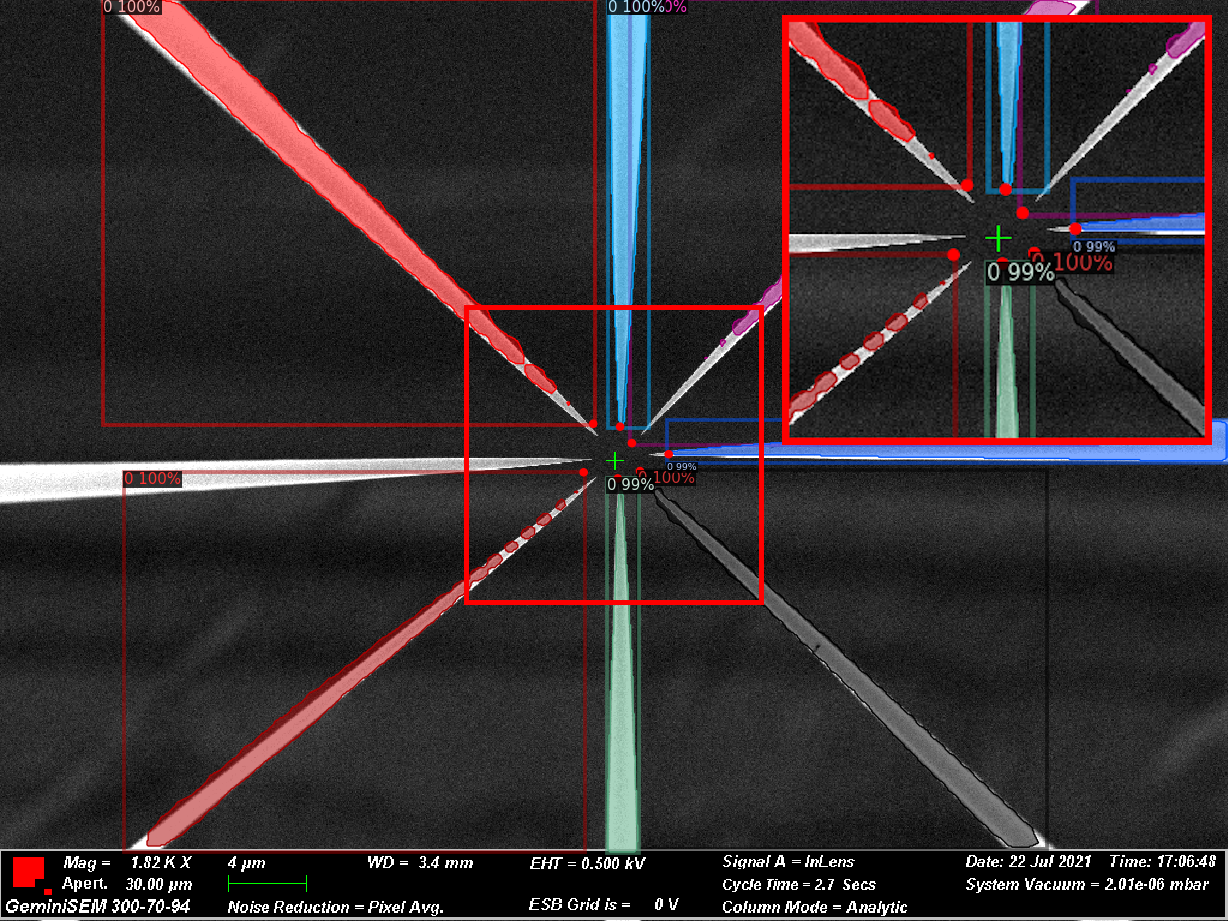
\includegraphics[width=0.485\textwidth]{img/eval/images/r50-dc5-image__004.png}}
    \subfigure[ResNet-101-FPN]{\label{subfig:r101-fpn-img2}
    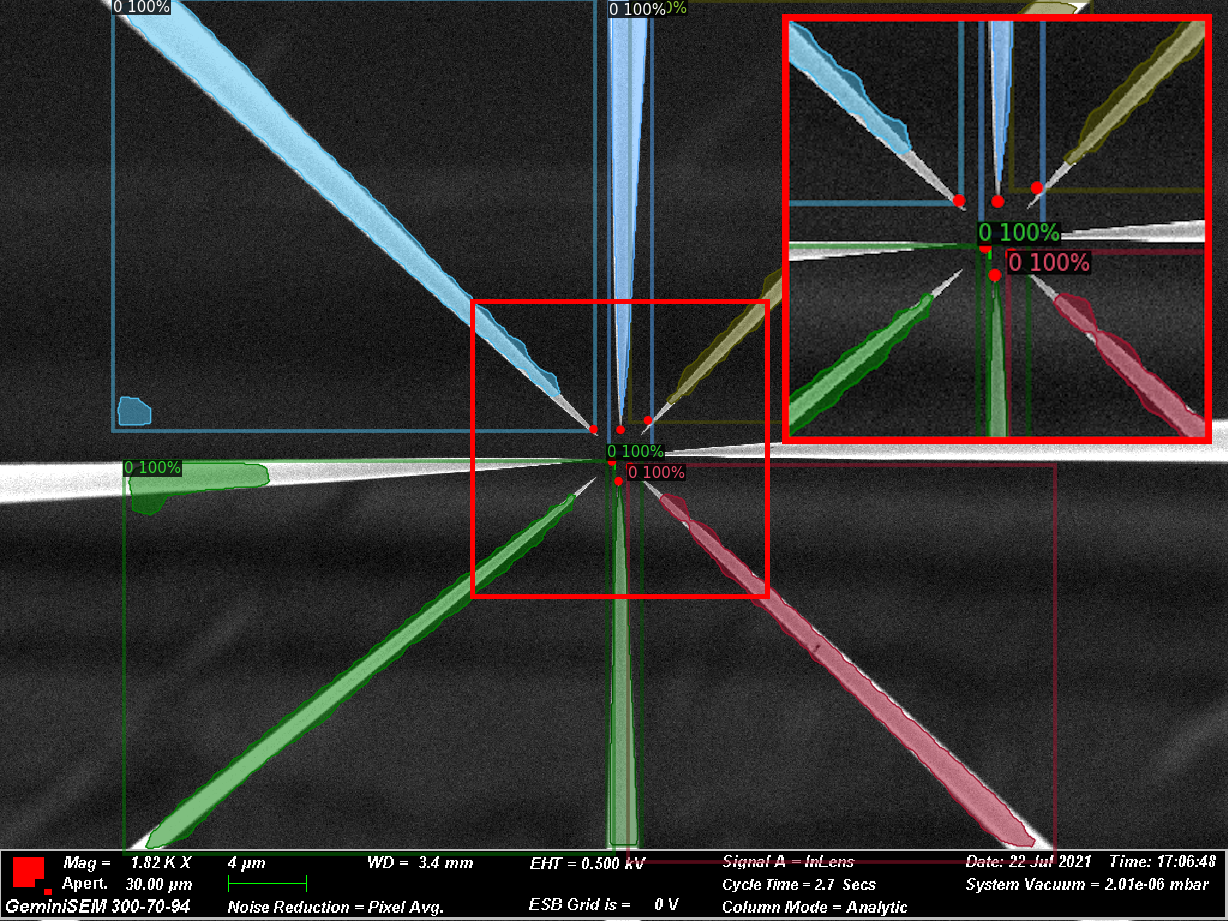
\includegraphics[width=0.485\textwidth]{img/eval/images/r101-fpn-image__004.png}}
    \subfigure[ResNet-101-DC5]{\label{subfig:r101-dc5-img2}
    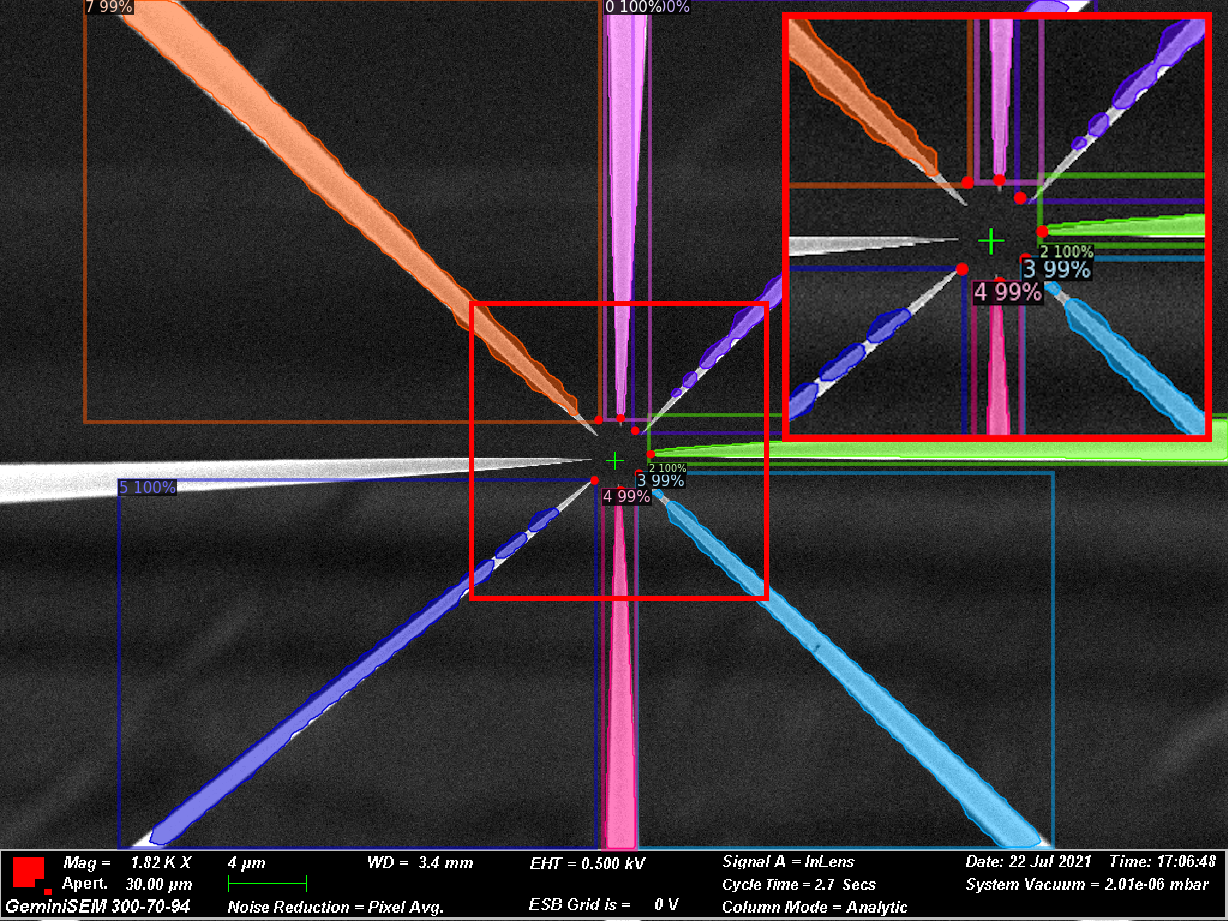
\includegraphics[width=0.485\textwidth]{img/eval/images/r101-dc5-image__004.png}}
    \caption{Segmentierung und Keypoints der verschiedenen Netzvarianten. Aufgenommen bei 2.000-facher Vergrößerung. Der zentrale Bereich ist vergrößert dargestellt.}
    \label{fig:comp_img2}
\end{figure}
Bei Vergrößerungen im Bereich von $10^3$, bei der die Nadeln lang, schlank und spitz erscheinen (siehe Abbildung \ref{fig:comp_img2}), zeigen die Modelle ein ähnliches Verhalten. Vereinzelt werden Nadeln gar nicht oder nur bei einer Konfidenz im Bereich von 90\% bis 98\% erkannt. Die Modelle haben Schwierigkeiten, den vorderen Teil der Spitze korrekt zu segmentieren. Teilweise hört die Segmentierung vor dem vordersten Punkt auf oder die Umgebung wird der Spitze zugeordnet.
Die vorher beobachtete wellenförmige Segmentierung der Eckspitzen, führt bei Vergrößerungen im Bereich von 1000 bis 5000x zu einer sogenannten \glqq Inselbildung\grqq{} in der Segmentierung des vorderen Spitzenbereichs.
Die FPN-Varianten der Modelle leiden bei der Segmentierung in diesen Szenarien unter Artefakt Bildung.

Die quantitative Messung der Genauigkeit spiegelt sich in der Keypoint-Vorhersage wider: Die DC5-Varianten der Modelle erzeugen genauere Keypoint-Vorhersagen als die FPN-Varianten. Ebenso bestätigt sich, dass die ResNet-101-Variante des Backbones zu einer genaueren Identifikation der Keypoints beiträgt.
\newpage
\begin{figure}[h!]
    \centering
    \subfigure[ResNet-50-FPN]{\label{subfig:r50-fpn-img1}
    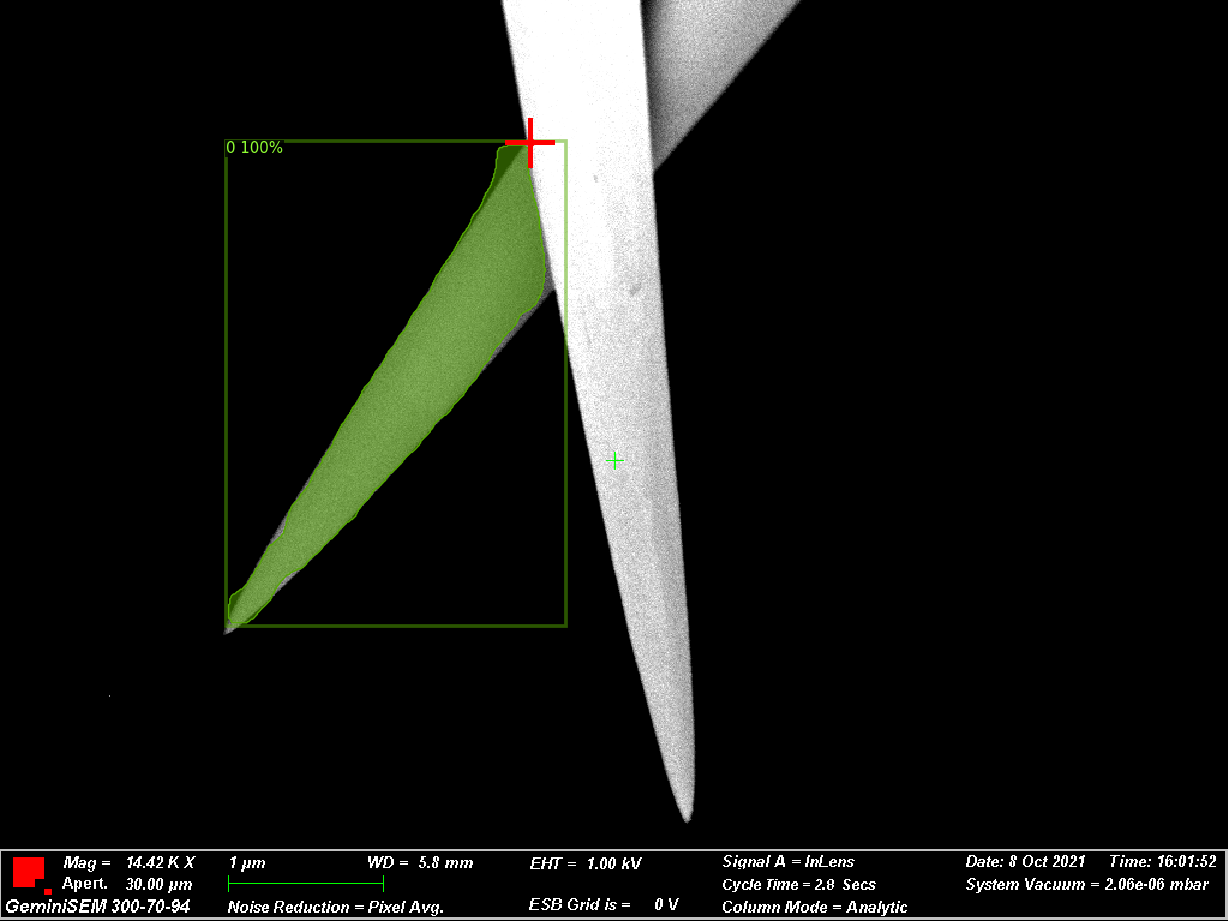
\includegraphics[width=0.485\textwidth]{img/eval/images/r50-fpn-Xilinx_n1_108.png}}
    \subfigure[ResNet-50-DC5]{\label{subfig:r50-dc5-img1}
    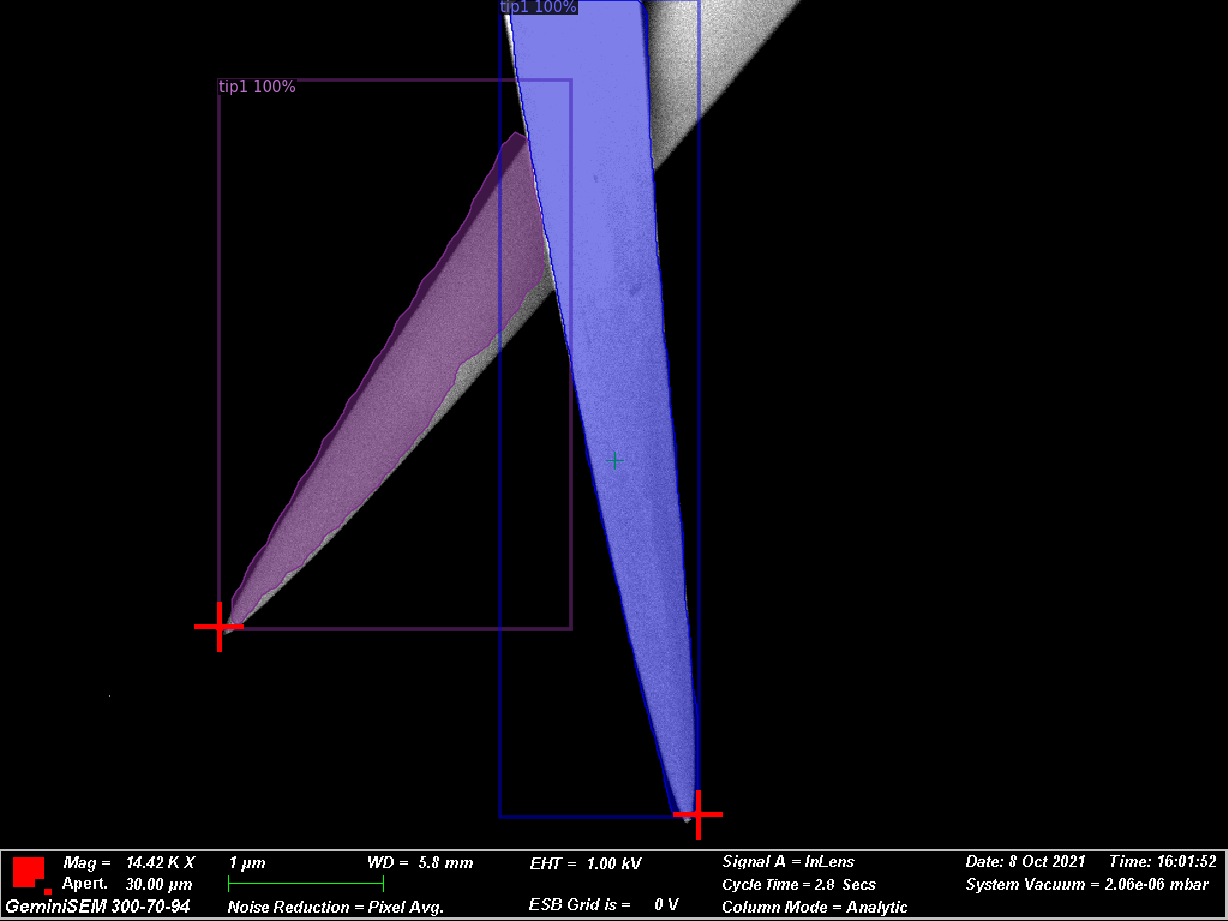
\includegraphics[width=0.485\textwidth]{img/eval/images/r50-dc5-Xilinx_n1_108.png}}
    \subfigure[ResNet-101-FPN]{\label{subfig:r101-fpn-img1}
    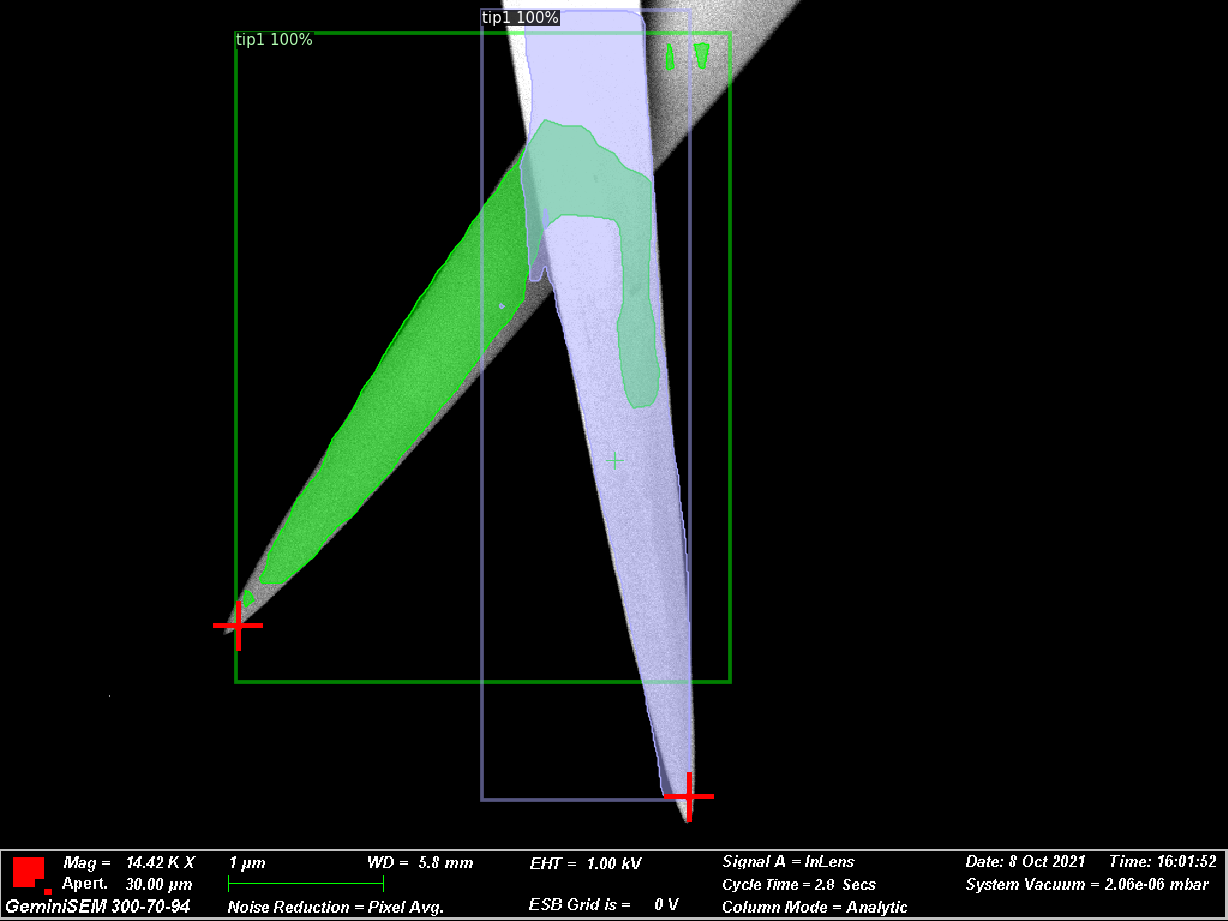
\includegraphics[width=0.485\textwidth]{img/eval/images/r101-fpn-Xilinx_n1_108.png}}
    \subfigure[ResNet-101-DC5]{\label{subfig:r101-dc5-img1}
    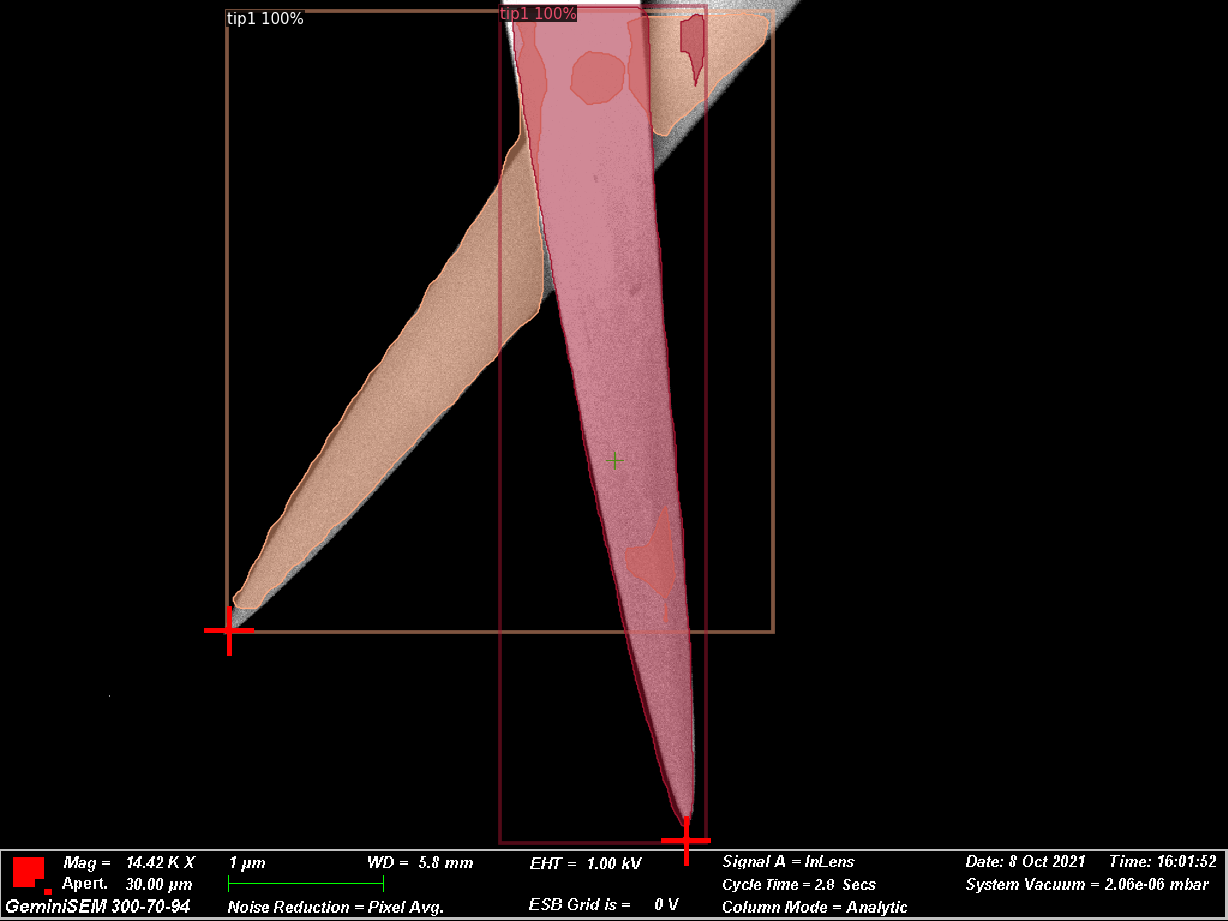
\includegraphics[width=0.485\textwidth]{img/eval/images/r101-dc5-Xilinx_n1_108.png}}
    \caption{Zwei gekreuzte Nadeln, dieses Szenario tritt bei der Reinigung der Spitzen auf.}
    \label{fig:comp_img3}
\end{figure}
Abbildung \ref{fig:comp_img3} zeigt die Spitzen in einem speziellen Szenario. Dem sogenannten Tip-Cleaning. Dabei überlagern sich zwei Nadeln. Diese Situation stellt eine besondere Herausforderung dar, da eine Spitze in zwei nicht zusammenhängenden Teilen des Bildes dargestellt wird und das Modell ein gewisses Verständnis dafür haben muss, dass Spitzen kontinuierlich verlaufen und nicht abrupt enden.
Keines der Modelle lieferte in dieser Situation robuste Detektionen. Sie weisen Fehler auf, die von falsch-negativen Erkennungen über Teilerkennungen bis hin zu Mehrfacherkennungen der Spitze reichen, bei denen die beiden Teile als unabhängige Nadeln angesehen werden. Das Modell ResNet-50-FPN ist in keinem der Bilder in der Lage, die Kontinuität der Nadel zu erkennen.
Die Modelle ResNet-50-DC5 und ResNet-101-FPN zeigen hingegen erste Erfolge: In Einzelfällen sind sie in der Lage, zwei sich überlappende Nadeln als zusammenhängend zu segmentieren, wenn auch nicht mit hoher Genauigkeit. Das Modell ResNet-101-DC5 liefert am häufigsten eine zusammenhängende Segmentierung und kann eine gute Segmentierung liefern, wenn die Nadeln in einem Winkel von 90 Grad zueinander stehen.

\chapter{Diskussion der Modellleistung}
Ziel dieser Arbeit ist es zu untersuchen, inwieweit Deep Learning Modelle wie Mask R-CNN für die Spitzenerkennung in REM Bildern eingesetzt werden können.
Insbesondere die schwierigen und sich ständig ändernden Bildbedingungen stellen dabei eine besondere Herausforderung dar.
In den folgenden Abschnitten werden die Stärken und Schwächen der trainierten Modelle durch eine Diskussion der vorgestellten Ergebnisse aufgezeigt. 
\section{Wahl des Backbones}
Die Ergebnisse zeigen, dass die Verwendung von Dilated Convolutions zu einer signifikanten Verbesserung der Modellleistung in allen Bereichen führt. Eine Hypothese ist, dass die Modelle aufgrund der Einfachheit und Einheitlichkeit der Konturen und Spitzen erheblich von der Vergrößerung des rezeptiven Feldes profitieren. Durch die Einbeziehung von weiter entfernten Pixeln in die Kontextinformation kann deutlicher zwischen der Probenstruktur im Hintergrund und der Spitze unterschieden werden, auch wenn der Übergang in einigen Szenarien optisch fließend ist.

Eine signifikante Verbesserung der Leistung durch die Verwendung des komplexeren Backbones ResNet-101 anstelle von ResNet-50 kann aus den Ergebnissen nicht abgeleitet werden. Es sollte eine vorsichtige Abwägung zwischen der Modellleistung und dem erhöhten Rechenaufwand sowohl für das Training als auch für die Inferenz des Modells vorgenommen werden. Weiterhin sollte analysiert werden, inwieweit der Unterschied in den FN- und FP-Raten zwischen ResNet-50 und ResNet-101 durch mehr Trainingsdaten und eine Anpassung des Konfidenzschwellenwertes ausgeglichen werden kann.

Die folgenden Abschnitte der Diskussion beziehen sich nur auf die DC5-Varianten der Modelle.
\section{Wahrheitswert der Vorhersagen}
Wie eingangs erwähnt, ist die Minimierung von Fehlklassifikationen von großer Bedeutung, da diese zu erheblichen Schäden führen können. Die FN-Rate der auf eine Klasse trainierten Modelle liegt bei etwa acht Prozent. Dies ist für eine vollautomatische Steuerung nicht ausreichend. Mit der durchgeführten Evaluierung an einem einzelnen Datensatz kann nicht näher analysiert werden, unter welchen Bedingungen diese falsch-negativen Detektionen auftreten. Aufschluss kann hier die Erstellung mehrerer kleiner Datensätze geben, die speziell für einen Szenentyp erstellt werden. Auf diese Weise können problematische Bedingungen, unter denen falsch-negative Detektionen auftreten, identifiziert werden.

Die FP-Rate der Modelle liegt bei ca. vier Prozent. Dies sind bereits gute Werte und zeigen die Resistenz der Modelle gegenüber spitzenähnlichen Strukturen. Hier können jedoch durch eine detaillierte visuelle Inspektion Hintergrundstrukturen erkannt werden, die vom Modell fälschlicherweise als Spitze erkannt werden. Durch ein nachträgliches gezieltes Training auf diese Strukturen kann die FP-Rate vermutlich noch weiter gesenkt werden.

Da bekannt ist, wie viele Spitzen auf dem Prober Shuttle montiert sind, können viele falsch-positive Detektionen herausgefiltert werden, indem nur die entsprechende Anzahl von Detektionen mit den höchsten Konfidenz werten verwendet wird.
Mehrfachdetektionen einer Spitze sollten durch die Verwendung eines Schwellenwertes, der das Überlappungsverhältnis der Segmentierungen von zwei detektierten Peaks regelt, herausgefiltert werden können. Wenn dieser Wert nahe bei 1 liegt, handelt es sich mit hoher Wahrscheinlichkeit um eine Mehrfachdetektion.
\section{Leistungssteigerung durch Richtungsvorhersage}
Die Gesamtleistung der Modelle verbesserte sich durch die zusätzliche Klassifizierung der Spitzen nach ihrer Richtung. Dies ist ein großer Vorteil, da die nachträgliche Zuordnung der detektierten Spitzen zum jeweiligen Manipulator bereits erledigt ist. Insbesondere die Segmentierung der Spitzen profitiert davon. Es wird vermutet, dass dies daran liegt, dass jeder der acht Maskenzweige des Modells auf eine bestimmte Form spezialisiert ist und eine Rotation der Spitze bei der Rekonstruktion aus den extrahierten Merkmalen nicht berücksichtigen muss.

Es wird angenommen, dass der positive Einfluss auf die FN- und FP-Raten darauf zurückzuführen ist, dass durch die Unterscheidung der acht Spitzen weniger Hintergrundstrukturen vorhanden sind, die aus einer Mischung von Merkmalen der acht Spitzen bestehen und daher fälschlicherweise als diese erkannt werden. Die Spitzen werden weniger verallgemeinert. Daher ist eine genauere Übereinstimmung mit einer Spitze aus einer bestimmten Richtung erforderlich.

In diesem Fall können auch einige Annahmen über die Detektionen getroffen werden.
\begin{itemize}
    \item Es können nur Spitzen detektiert werden, die montiert sind.
    \item Es kann maximal eine Spitze jeder Klasse detektiert existieren.
    \item Die acht Spitzen haben alle einen vordefinierten Randbereich, aus dem sie in das Bild ragen. 
\end{itemize}
Durch diese Vorannahmen sollte es möglich sein, die FN- und FP-Raten der Modelle durch nachträgliches Filtern zu minimieren.

Die in Abbildung \ref{tab:correl} dargestellten Korrelationskoeffizienten deuten auf einen komplexen Zusammenhang zwischen der Modellleistung, der Anzahl der Trainingsbilder pro Klasse und der Eckposition hin.
Um hier einen tieferen Einblick zu erhalten, sollte ein Datensatz erstellt werden, in dem die Anzahl der Instanzen pro Spitze gleich verteilt ist. Dadurch kann der Zusammenhang besser analysiert werden. Eventuelle Schwächen können so auch durch ein anschließendes Feintraining des Modells gezielt angegangen werden.
\section{Qualität der Segmentierung}
Die durch das Modell erzeugte Segmentierung der Spitzen erweist sich bei der visuellen Überprüfung als sehr situationsabhängig. Bei Vergrößerungen über 10.000 ist sie nahezu perfekt. Bei Vergrößerungen unter 10.000 ist die Segmentierung zur Spitze hin ungenau. Hier ist eine weitere Evaluierung der Modelle anhand von Datensätzen unterschiedlicher Vergrößerungsstufen erforderlich. Es ist jedoch davon auszugehen, dass Mask R-CNN aufgrund der Kompression der Bilddaten bei der Merkmalsextraktion nicht für eine qualitativ hochwertige Segmentierung sehr feiner Strukturen geeignet ist.

Ein Ansatz zur Lösung des Problems der unsauberen Segmentierung der Eckpunkte besteht darin, das Bild zweimal durch das Modell verarbeiten zu lassen. Einmal im Original und einmal um 45 Grad gedreht. Die resultierenden Segmentierungen können zusammengeführt werden, um eine genaue Segmentierung aller Spitzen zu erhalten. Dies erfordert jedoch eine schnelle Bildverarbeitung, da die zu verarbeitende Bildrate verdoppelt wird.

Die nachträgliche Analyse des Datensatzes \glqq 750img\_merged\grqq{} ergab, dass sich unter den Bildern nur 14 Bilder mit sich kreuzenden Spitzen befinden, die meist im 90-Grad-Winkel zueinander stehen. Vor diesem Hintergrund ist es erstaunlich, dass die Modelle in einigen Szenen in der Lage sind, sich kreuzende Spitzen korrekt zu segmentieren. Um jedoch Prozesse wie das Tip-Cleaning automatisieren zu können, sollte der Datensatz erweitert werden.

Da eine pixelgenaue Segmentierung nicht so wichtig ist wie eine zuverlässige Erkennung, kann man sagen, dass die Qualität der Segmentierung in den meisten Fällen mehr als ausreichend ist.
\section{Genauigkeit und Probleme der Keypoint-Vorhersage}
Bei kleinen Vergrößerungen, insbesondere bei Vergrößerungen unter 10.000, weichen die vorhergesagten Positionen von der Realität ab. Die Analyse der Abweichungen zeigt, dass diese normalverteilt sein können, wodurch die Ungenauigkeit durch eine Varianz charakterisiert werden kann. Die Bestimmung der Varianz ermöglicht es, für die Vorhersage einen Konfidenzbereich anzugeben, der die Wahrscheinlichkeit umfasst, dass die wahre Position innerhalb eines bestimmten Intervalls liegt.

Die Verwendung einer Normalverteilung in dieser Analyse hat den zusätzlichen Vorteil, dass sie eine statistische Grundlage für die sichere Steuerung der Manipulatoren bietet, auch wenn die Vorhersagen ungenau sind. Durch die Quantifizierung der Unsicherheit kann die Steuerung entsprechend angepasst und optimiert werden, um mögliche Fehler zu minimieren.

Ein Ansatz zur Verbesserung könnte darin bestehen, die grobe Erkennung zu verfeinern, indem der nachträglich vergrößerte Bildbereich erneut verarbeitet und die Informationen zusammengeführt werden. Diese Methode könnte die Genauigkeit in Situationen mit geringer Vergrößerung erhöhen.

Die erreichte Genauigkeit bei der Lokalisierung des vordersten Punktes der Spitzen ist jedoch insgesamt von hoher Qualität. Die quantitativen Ergebnisse, die einen $\text{AP}^{OKS=.75}$ von über 95\% zeigen, werden durch die optische Überprüfung bestätigt. Es ist beeindruckend, dass selbst für Spitzen, deren vordere Struktur mit der darunter liegenden Probenstruktur verschmilzt, die Vorhersagen genau sind.

% \begin{figure}[htbp]
%     \centering
%     \subfigure[]{\label{subfig:}
%     \includegraphics[width=0.32\textwidth]{}}
%     \subfigure[]{\label{subfig:}
%     \includegraphics[width=0.32\textwidth]{}}
%     \subfigure[]{\label{subfig:}
%     \includegraphics[width=0.32\textwidth]{}}
%     \subfigure[]{\label{subfig:}
%     \includegraphics[width=0.32\textwidth]{}}
%     \caption{}
%     \label{fig:}
% \end{figure}